\chapter{Гора, Замковая, Воловня}

Прогуляемся по киевским горам, связанным с летописными князьями полянскими, а также осмотрим окрестности. Пойдем от фуникулера  Десятинной улицей в сторону Андреевской церкви.

Шагая по Десятинной, мы перемещаемся по Горе. Она же Киевская и Старокиевская. Вероятно, холм сей в летописное время именовали Киевицей. Ибо Кий жил, «идеже ныне», при Несторе, увоз Боричев.

Под Киевицей могли подразумевать и б\'ольшую часть горы, включавшую Замковую и Клинец, которые тогда почти не отделялись от общего кряжа. Серое огромное здание МИД (где раньше стояла Трехсвятительская церковь на месте идолов), дома вдоль улицы Десятинной – это всё Гора.

В отличие от науки, я не считаю, что на Горе были княжьи дворы Ольги, Владимира и многих других князей, поэтому введенные в обиход представления о «граде Владимира» и о древнем Киеве, где-то тут уместившемся на пятачке земли, для меня лишены смысла. Но заблуждения буду развеивать по мере надобности.

Горы касаюсь во многих главах – про Боричев, про Вольгу. Здесь же поведаю о замке, а точнее, дороге сквозь него, да горе Клинец, которую все потеряли, а я взял да нашел.

Пока мы не дошли до Андреевского спуска, кое-что обсудим. Задумчивым жестом, словно экскурсовод, указываю на асфальт.

Под Десятинной улицей, на большой глубине, была пещера. Провал в нее обнаружил в 1838 году Александр Семенович Анненков, курский и орловский помещик, сосланный в двадцатые годы 19 века в Киев за жестокое обращение с крепостными крестьянами. Тут Анненков завязал знакомства с любителем древностей митрополитом Евгением (Болховитиновым) и археологом-мистиком Лохвицким, и приобрел усадьбу возле участка, на котором, как считают, стояла древняя Десятинная церковь.

Анненков пожелал выстроить там новую церковь взамен поставленной еще Петром Могилой, а заодно принялся усердно раскапывать окрестности. При этом Болховитинов следил за археологическими находками, и они в итоге стали достоянием церкви и науки.

Но в 1842 году строительство завершилось, надзор сняли. Тогда-то Анненков отрыл по соседству клад золотых и серебряных предметов, объемом в два мешка. Либо оные предметы он утаивал ранее, а теперь решил перепрятать. Сокровища Анненков отправил на свой хутор в Полтавской губернии.

Предание гласит, что часть древностей была перелита в слитки, часть же досталась неграмотным крестьянам – и они-то использовали старинные браслеты как собачьи ошейники, а прочие украшения отдали для забав детям. История с дремучими крестьянами кажется мне баснословной. 

Так вот, этот Анненков во время перекапывания всех околиц нашел возле Трехсвятительcкой церкви лаз, ведущий в глубокую пещеру, прорытую в лёссе. Пещера имела своды, подобные лаврским пещерам, и несколько ветвей, исследовать которые до конца не удалось – коридоры оказались засыпаны, а дальше и не рыли.

Что с этой пещерой теперь, неясно, равно как и с пещерами Михайловского монастыря. Не знали о таких?

Как известно, Михайловский монастырь, что стоит сейчас над Боричевым – построен заново в конце девяностых, а снесен был в 1930-х. Осталась впрочем трапезная церковь Иоанна Богослова и гостиницы для паломников, служившие потом общагами студентам. В 1965 году среди превращенной в парк бывшей усадьбы монастыря энтузиасты наткнулись на входы в пещеры. Некоторые отверстия были засыпаны, иные заложены кирпичами, вероятно в 17 веке.

При редакции газеты «Вечерний Киев» на общественных началах действовала комиссия по изучению подземелий. Это ее члены годом раньше провели раскопки в Церковщине. И вот на волне интереса, они бросили все силы на бывшую усадьбу Михайловского монастыря.

Несколько дней исследователи воодушевленно расчищали подземные ходы, но своими силами далеко зайти не удалось, а официальная наука почин не поддержала. С тех пор про пещеры под Михайловским Златоверхим ничего не слышно.

Вообще Верхний город обычно не связывается с пещерами, между тем весь пронизан ими, как шляпка червивого гриба. В 19 веке нашли коридор, шедший под землей к Золотым воротам от нынешней улицы Лысенко. Его расчистили на длину около ста метров. Подобный же ход, укрепленный сосновыми бревнами, отыскал Викентий Хвойка в 1908 году в усадьбе Петровского, где сейчас Исторический музей.

Время от времени подземелья открываются в окрестностях Софии. В 1916 году к северо-западу от нее образовался провал в коридор, высотой около двух метров и шести длиной. Внутри лежали французская медная монета времени Людовика XIV (17 век), битый кирпич того же века, но также и древнерусские кирпичи – плинфа, да куски сланца (археологи называют его шифером). Там были ниши с люками, смотрящими вверх. От главного коридора шел в сторону другой. Подземную полость проследили бурением скважин до перекрестка Стретенской с Малой Владимирской (Чкалова, Гончара). Пещеру исследовал Эртель, предположивший, что разные части ее выкопаны в разное время. 

Ученых озадачило подземелье – для чего оно предназначено? Эти ниши, люки... А меня озадачивает сообщение из дневника Эриха Ляссоты, посланца императора Рудольфа к запорожским казакам. Ляссота проезжал через Киев в 1594 году, посетил и Софию. Он пишет\cite{sbornikmat}:

\begin{quotation}
Вверху церкви есть галерея, или верхнее отделение церкви; перилы этой галереи, от одного столба до другого, из цельных плит голубоватого камня, с резной отделкой. Из них одна плита, что напротив главного алтаря, имеет круглое отверстие, примерно в пол-локтя, которое теперь заделано известью.

Говорят, что в этом отверстии прежде находилось зеркало, в котором, посредством искусстве магии, можно было видеть все, о чем бы ни задумали, хотя бы то за несколько сот миль.

Но случилось следующее: один киевский царь отправился на войну в языческую землю и долго оттуда не возвращался; а жена его с тоски по мужу имела обыкновение ежедневно смотреть в это зеркало, желая знать, что делает ее господин и как ему там живется.

Увидев однажды в зеркале, между прочим, что муж ее любезничал с пленною язычницею, она в сильном гневе разбила зеркало: sit fides penes autorem\footnote{В переводе – мол, сказанное остается на совести рассказчика.}.
\end{quotation}

Я верю этому рассказу и понимаю его буквально, как верю в существование дисплеев и видеокамер, при помощи которых люди общаются между собой, будучи разделенными «многими милями». Однажды киевский князь просто забыл выключить камеру. Ну а вопрос, откуда в то давнее даже для 16 века время взялись подобные технологии – это ученых не озадачивает, равно как и сия выдержка из дневника Ляссоты.

И снова о подземельях. В 1925 году, как обычно случайно, провалилась земля и открылась новая пещера возле Софии. Раскопками занялся Василий Ляскронский. В начале пещеры находилось облицованное кирпичом помещение, затем коридор уходил в лёсс. Куда именно -неведомо, ибо Ляскронский отложил дальнейшие изучение сначала на год, а потом навсегда.

Осенью 2014-го археологи проводили в Софии раскопки каменного сооружения, трактуемого ими как «остатки храма 11 века». Около стены этого здания была пристройка с подземной частью, обложенной бревнами. Полагают, что усыпальница. Там в полу был уходящий в лёсс проход, его расчистили на шесть метров. Продолжить решили в следующем году. Чем всё закончилось, не знаю. 

Пока я это рассказывал, мы дошли до Андреевского спуска. Ниже Андреевской церкви, и чуть ниже дома Ричарда Львиное Сердце\footnote{Построенный в начале 20 века на средства купца Орлова, был доходным домом, после революции в нем разместились коммунальные квартиры. Предание гласит, что вдова Орлова расплатилась со строителями несправедливо, и те «поселили» в дом привидений, насыпав в дымоход яичную скорлупу. Её нашел там профессор Киевской Духовной академии Степан Тимофеевич Голубев и объяснил, что воздух, проходя через мелкие дырочки в скорлупе, вызывал те странные звуки, что пугали обитателей дома и создавали оному дурную славу.}, будут две горы, на кои ведут крутые лестницы.

К востоку, со стороны Днепра – небольшая гора с ровно обрезанной верхушкой. Это Уздыхальница, ранее Здыхальница. В 19-м и начале 20-го веков, весь склон по верху от Боричева до Уздыхальницы называли Андреевской горой. А иногда так именовали только отдельный холмик с Андреевской церковью. Я избегаю употреблять это смутное название – Андреевская гора. По преданию, на одном из отрогов Горы апостол Андрей установил крест.

В различных источниках сказано так: «И крест святый на них, где теперь церковь святого Семиона стоит, поставил», «Идеже ныне церковь воздвижения креста господня», «а потом вшедши на гору, подле которой теперь стоит брама Киевская замковая на полудне (юг) и церковь воздвижения креста святого», «на той тогда горе в Киеве, идеже святыи андрей стоял, юже нарицают вздыхальницу, в тоже время и церковь воздвижения пречестнаго креста господня была поставлена, идеже и ныне есть».

Чуть дальше Уздыхальницы и к западу... А вот тут заковырка.

\begin{center}
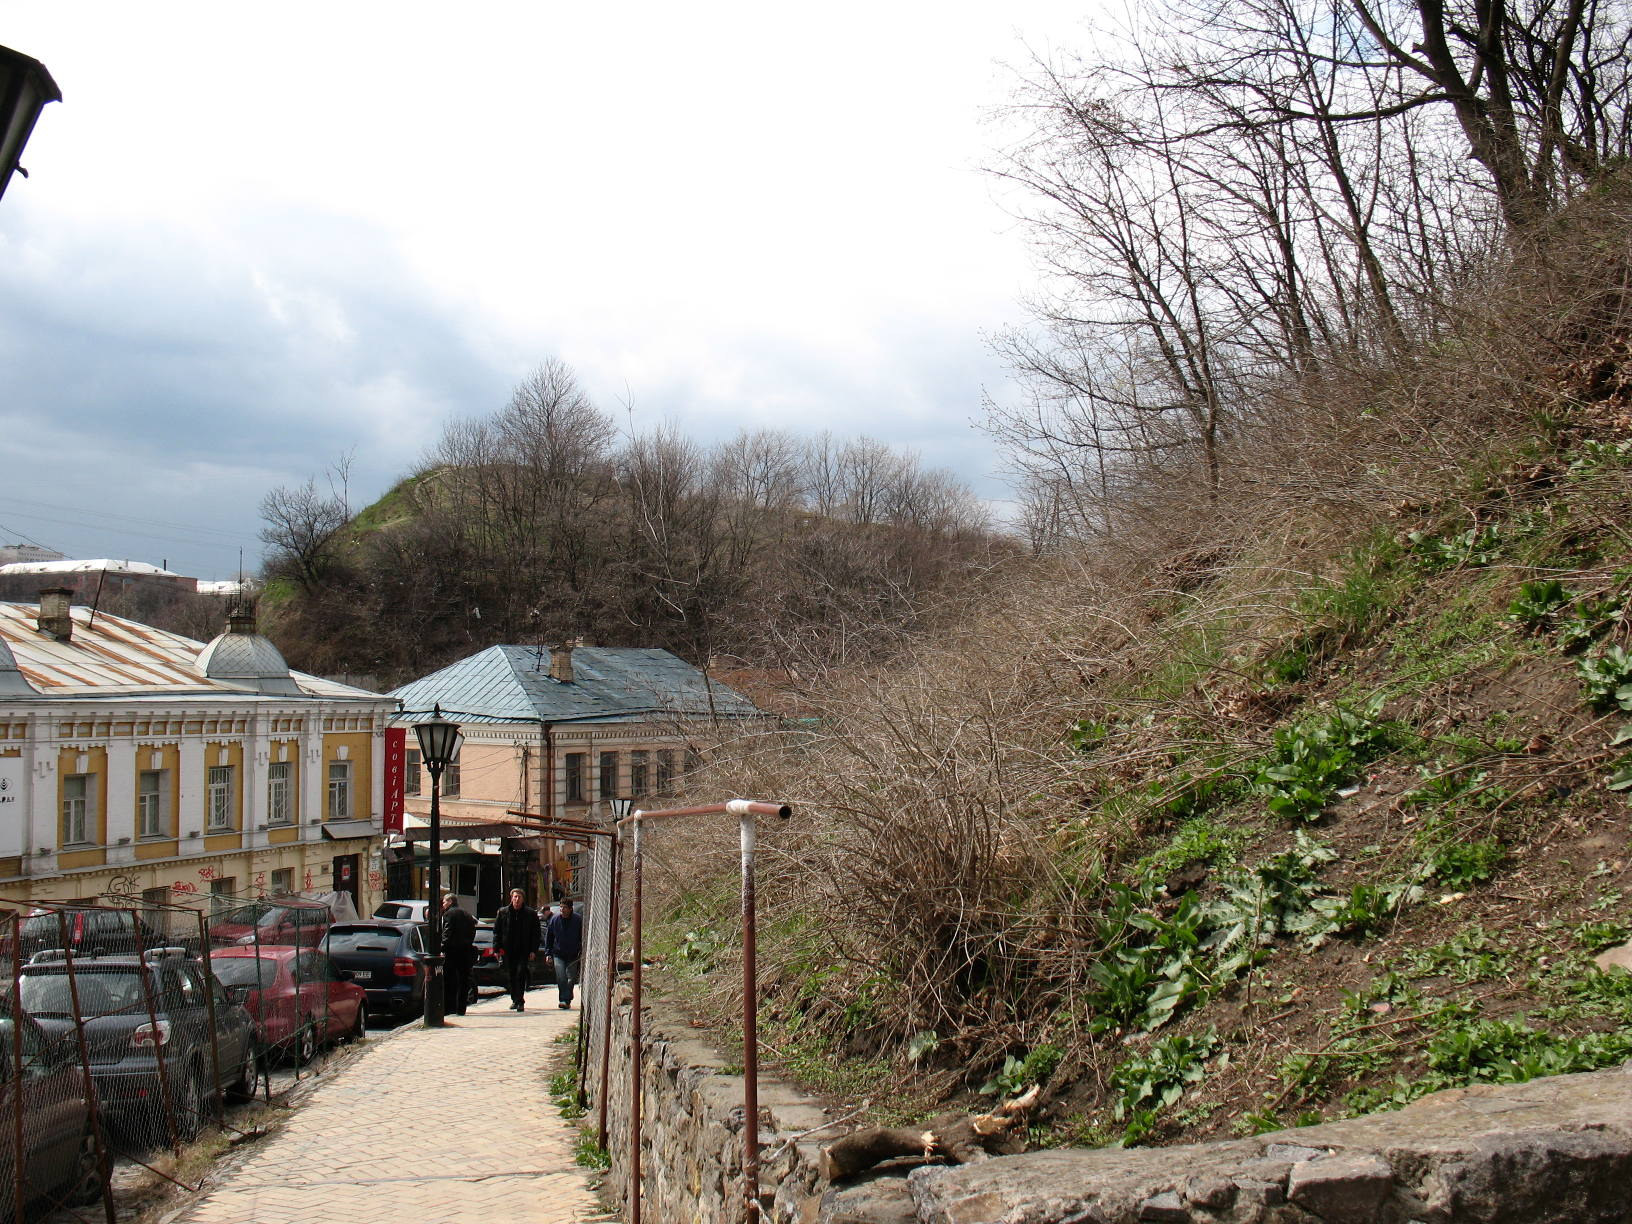
\includegraphics[width=\linewidth]{chast-colebanie-osnov/gora-zamkovaya-valovaya/s_IMG_1195.JPG}
\end{center}

Обычно сию гору, похожую на двугорбого верблюда, называют Замковой, или же Киселёвкой, Флоровской, а иногда Хоревицей – последнее ошибочно. Я же докопался, что первый, южный горб, раньше слыл горой Клинцом. Затем в обиходе Клинец совместился с Киселёвкой. Поначалу же холмы различались. На предшествующем снимке, спереди – Клинец (теперь – южный горб Киселёвки), справа – склон Уздыхальницы.

С высоты полета, Замковая гора и Уздыхальница, разделенные Андреевским спуском, выглядят прямоугольником. Более того, ровно подрезан и северо-восточный склон следующей горы, Щекавицы, продолжая линию того же склона Замковой!

На Замковой горе стоит камень с современной надписью, что это «Хоревица». Летописи не оставили на сие указаний, а древнее народное название утеряно. Из тьмы веков, гора проявляется в источниках как Замковая и Киселёвка.

\newpage
\vspace*{\fill}
\begin{center}
\includegraphics[width=\linewidth]{chast-colebanie-osnov/gora-zamkovaya-valovaya/\myimgprefix aspusk.jpg}

\textit{Андреевский спуск на стыке 19-20 веков. Прямо, со шпилем – дом Ричарда, за ним видна Киселёвка.}
\end{center}

\begin{center}
\includegraphics[width=\linewidth]{chast-colebanie-osnov/gora-zamkovaya-valovaya/\myimgprefix zamdet.jpg}

\textit{19 век. Слева – гора Детинка, справа с церковью – Замковая. Дома в удольи – урочище Гончары и Кожемяки.}
\end{center}
\vspace*{\fill}
\newpage

\vspace*{\fill}
\begin{center}
\includegraphics[width=0.95\linewidth]{chast-colebanie-osnov/gora-zamkovaya-valovaya/\myimgprefix klinec.jpg}

\textit{19 век, вид с другой стороны, со горы Воловни (где Вознесенский спуск). Слева – Клинец, справа – Детинка. Дома на переднем плане – Дегтярная улица.}
\end{center}

\begin{center}
\includegraphics[width=0.95\linewidth]{chast-colebanie-osnov/gora-zamkovaya-valovaya/\myimgprefix zamdet02.jpg}

\textit{19 век, вид с Замковой. Справа – Детинка. Внизу всё те же Гончары и Кожемяки. Эти домики простояли до 1980-х.}
\end{center}
\vspace*{\fill}
\newpage

Однако, от неё внизу отходит улица Хоревая, известная по крайней мере с начала 19 века. Почему так решили назвать улицу? Непрерывное народное предание, известное тем, кто нарёк улицу? Но в старинных земельных документах нет «Хоревицы». «Хоревица» в связи с Замковой выползает ближе к окончанию 20 века усилиями популяризаторов и журналистов, которые любят проводить маленькие, короткие изыскания и делать быстрые выводы.

В Киеве существует улица Предславинская, названная по летописному «сельцу Предславино», где жила Предслава – дочь Рогнеды, жены Владимира. Согласно летописи, сельцо находилось на берегу речки Лыбеди, а улица Предславинская лежит от Лыбеди в 600 метрах! А вот Иван Иванович Мовчан полагал, что в ходе археологических исследований нашел Предславино в усадьбе дома 57 по улице Красноармейской – это к северу от Предславинской, на том же расстоянии от Лыбеди. Может быть, откопали древнерусскую табличку, висячий знак, как на трактире, с надписью «Предславино»? Нет. Но археологи пишут, что нашли Предславино.

И потом удивительно, как спешат давать улицам «исторические» имена. Еще севернее дома 57 есть улица Рогнединская, ранее прозаично – Бульонная. Наверняка смекнули, что где-то рядом с Предславой  жила и Рогнеда. 

Впрочем в середине 19 века, местность между Кловским ручьем и Госпитальным укреплением называлась Бульонкой, а гора напротив Троицкого базара (площадь у Республиканского стадиона и сам стадион) – Рогнединской. Предшествовало ли такое имя Черепановой, либо Рогнединской горой считали часть нынешней Черепановой? Как давно Рогнединскую гору стали называть Рогнединской? Иными словами, по ней дали имя улице, или наоборот? Относительно «Черепановой» – при холме была усадьба киевского гражданского губернатора (1814-16 годов) Павла Сидоровича Черепанова.

Вернемся к Замковой горе. 

Название её «Киселёвка» – п\'озднее, в русских летописях не встречается. В документах времен Литвы и Польши, в казацких хрониках, эту гору пишут то Замковой, то просто Замком. Жил такой Адам Свянтольдович Кисель Брусиловский, назначенный польским правительством с 1641 по 1650 годы комендантом, а с 1650 по год своей смерти, 1653-й, Киевским воеводой (палатином)\footnote{Палатинат, или воеводство – административная единица вроде области. Таким образом Киселя назначили главой Киевского палатината.}. От него и название Киселёвка. При Киселе да и прежде на горе стоял замок, уничтоженный, когда Киев от Польши перешел к России.

\begin{center}
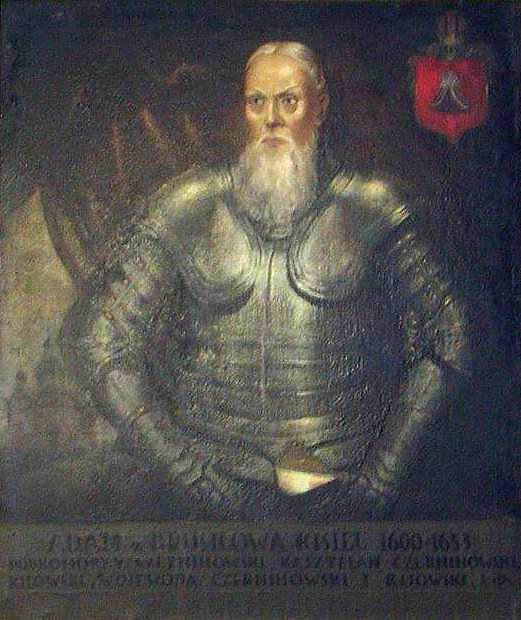
\includegraphics[width=0.40\linewidth]{chast-colebanie-osnov/gora-zamkovaya-valovaya/adam_kisiel.jpg}

\textit{Портрет Киселя.}
\end{center}

Замок был набором построек на плоском верху холма. Деревянная крепость, огороженная сосновым частоколом, перемежаемым деревянными же башнями с бойницами. В 1581 году Александр Гваньини, военачальник на службе у Польши, описывал его как «замок из дубов, камней и земли». Эрих Ляссота в 1594 году заметил: «Замок находится высоко на отдельной горе: он очень обширен, но не каменной постройки, а деревянный, оштукатуренный известью». Рейнольд Гейденштейн в 1596 году отзывался о замке так: «Над городом\footnote{Имеется в виду Подол.} господствует деревянный замок, но не стоит названия замка. Он совсем заброшен, и почти совершенно сгнил».

В первые десятилетия 21 века на горе, среди одичавших садовых деревьев – заброшенные остатки кладбища, некогда принадлежавшего Флоровскому женскому монастырю, что находится и процветает у восточного подножия горы\footnote{Поначалу просто Флоровский, он стал Флоровским Вознесенским после перевода сюда Вознесенского монастыря, что стоял напротив Лавры, где ныне «Мистецький арсенал».}. Поначалу здесь хоронили монашек, но, судя по надгробиям, с неких пор это правило было отменено и кладбище начало принимать также мужчин духовного звания, а быть может стало частично светским.

На кладбище была довольно большая Троицкая церковь. Нынче местность выглядит удручающе. Всюду ямы раскопанных могил, засыпанные листвою и мусором. Перекошенные кресты, разбитые каменные надгробия конца 19-го, начала 20-го веков. Валяется, со сбитой фотографией, надгробие Петра Ивановича Линицкого (1839-1896), профессора Киевской духовной академии, доктора богословия и сочинителя множества книг и статей по философии. Кто-то видел и его кости, разбросанные по склону. А от могилы Николая Петрова не осталось и следа.

Загадочный склеп, весь разрисованный и внутри загаженный. В 2005 году перед ним еще лежал большой и черный могильный камень – спустя шесть лет его уже не видно, и вообще некоторые надгробия стырили. На западной кромке горы сохранились остатки старой стены, окружавшей кладбище. Она построена в 1855-1857 годах из желтых и алых кирпичей с клеймами «КП I848», «КП I849», «КП I854», «КП I864», «КП 87I8», которые я трактую как клейма кирпичного завода Лавры, расположенного в пойме Лыбеди между Зверинцем и Лысой горой (Девич-горой).  

Некоторые могилы кем-то восстановлены, а таблички подновлены. Б\'ольшая же часть захоронений осквернена. Приведу здесь читаемые надписи по имеющимся у меня снимкам и статьям. Зачем это делаю? Быть может, кто-то из читателей отыщет среди фамилий своего предка. Кладбище разрушается, надгробий становится всё меньше. Надписи даю согласно современному правописанию. Знаки вопроса ставлю там, где не удалось разобрать.

Табличка: «Исаченко Антонина Мироновна 1913-43».

Табличка: «Флоровский м-рь ск.мон Мария (в миру Науменко Марина Васильевна) умерла в 1952 г.».

Табличка: «Пивень Мария Захаровна 1890-13.04.1950 Светлая память».

На могильном камне Яровенко эпитафия: «яко грядет час, и ныне есть, егда мертвии услышат глас Сына Божия и услышавше оживут. Иоан.5.25».

Надгробие: «Никита Николаевич Малиновский 1850 г. – 1904».

Надгробие: «? Симеона Лукича ВЛАДЫШЕВСКОГО род 8 Февраля 1834 г. Скон 21 Ноября 1902 Мир праху твоему дорогой муж».

Надгробие «Василий Петрович Наголкин скон 17 марта 1903 г. Дорогому Мужу и Отцу».

Надгробие:

\settowidth{\versewidth}{Остались нам на склоне дней.} 
\begin{verse}[\versewidth]
Мы погребли в могиле сей\\
Любовь, мечты и упованья\\
Остались нам на склоне дней\\
Одни лишь слезы и страданья.\\
\end{verse}

Надгробие: «? дочь ди? девица Мария Крамар ? блажении ме? мирающии о гос ?».

Надгробие: «Здесь покоится священик Андрей Иоаннович Жалобовский умер 21 Апреля 1907 г. На 70-м году».

Надгробие: «Петр Петрович Алексеев Род. 14-го Апреля 1840 г. Сконч. 6-го Февраля 1891 г.».

Надгробие: « …его Алексея Васильевича Губарева 
сконч. 6 Июля 1894 г. на 50 г. жизни Мир праху твоему дорогой Отец».

Надгробие: «…младенцы Андрей Мария Андрей
Вишневецкие Таковых есть царствие небесное».

Надгробие: «Под сим камнем погребено тело Натальи Ивановны Некрасовой ? 1882 года 15 Июля».

Надгробие: «Помяни Господи рабу Твою Марию!».

Посмотрим на фотографии, снятые на Замковой горе и около. Цветные относятся к 2011 году, черно-белые к дореволюционному времени.

\newpage
\vspace*{\fill}
\begin{center}
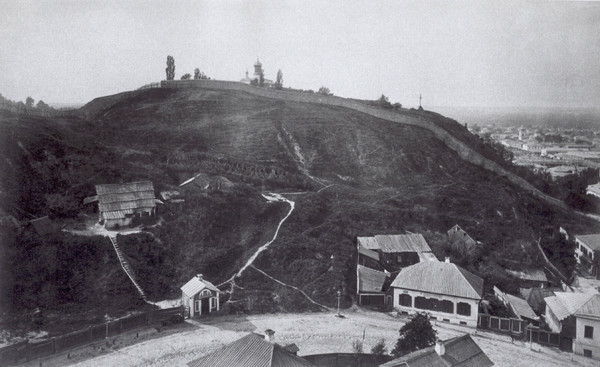
\includegraphics[width=\linewidth]{chast-colebanie-osnov/gora-zamkovaya-valovaya/zamkovaya_s_uzd.jpg}

\textit{Ракурс на Замковую гору с Уздыхальницы, конец 19 века. Видно стену, кладбищенскую церковь.}
\end{center}

\begin{center}
\includegraphics[width=\linewidth]{chast-colebanie-osnov/gora-zamkovaya-valovaya/\myimgprefix IMG_1213.JPG}

\textit{Тот же вид, 12 апреля 2011.}
\end{center}
\vspace*{\fill}
\newpage

\vspace*{\fill}
\begin{center}
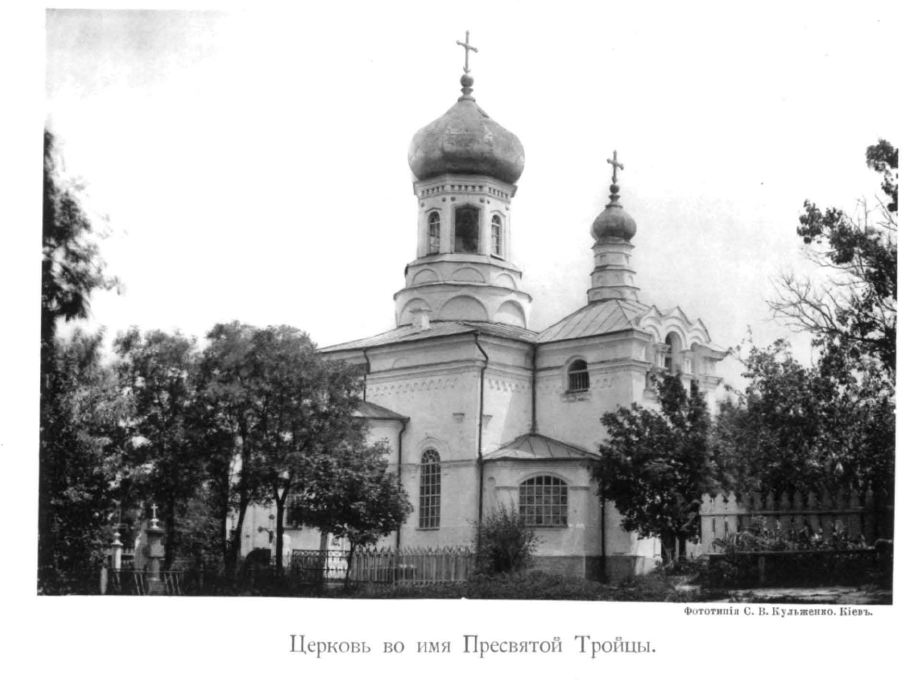
\includegraphics[width=\linewidth]{chast-colebanie-osnov/gora-zamkovaya-valovaya/kiselevka-troick-cerk-1894.png}
\end{center}

\begin{center}
\includegraphics[width=\linewidth]{chast-colebanie-osnov/gora-zamkovaya-valovaya/\myimgprefix IMG_1325.JPG}
\end{center}
\vspace*{\fill}
\newpage

\begin{center}
\includegraphics[width=\textwidth]{chast-colebanie-osnov/gora-zamkovaya-valovaya/\myimgprefix IMG_1350.JPG}
\end{center}

\begin{center}
\includegraphics[width=\linewidth]{chast-colebanie-osnov/gora-zamkovaya-valovaya/\myimgprefix IMG_1336.JPG}
\end{center}

Хотели бы современные варвары, чтобы с их могилами так поступили будущие поколения?

А вот старинная лестница, 1855-1857 годов, подновленная в советское время. Она идет по юго-восточному склону горы (если не считать Клинец за Киселевку) и спускается к началу улицы Флоровской, месту, где раньше была улица Черная грязь:

%\begin{center}
%\includegraphics[width=\linewidth]{chast-colebanie-osnov/gora-zamkovaya-valovaya/IMG_1313.JPG}
%\end{center}

\begin{center}
\includegraphics[width=\linewidth]{chast-colebanie-osnov/gora-zamkovaya-valovaya/\myimgprefix IMG_1380.JPG}
\end{center}

Сходя по этой лестнице, кажется, будто холм обнимает её правым, крутым своим склоном, иногда отходя в сторону. В землистую гору вцепились корнями деревья. Наверху – столб электропередачи да остатки перил из сваренных металлических труб. Там же, лестница пребывает в старинном состоянии. Поначалу это вымощенная светлым прямоугольным камнем дорожка с каймой из замшелого кирпича. Затем дорожка начинает понижаться и переходит в более современную, где каждые три ступени чередуются с бетонной плитой, а справа, из обмазанных цементом кирпичей сделан заградительный бугор, чтобы склон не наползал на лестницу. Кое-где, у террас, в опавшей листве виднеются груды старых кирпичей, некие фундаменты, засыпанные давними оползнями.

Внизу лестницы, в 2011 году картина была такая:

\begin{center}
\includegraphics[width=0.80\linewidth]{chast-colebanie-osnov/gora-zamkovaya-valovaya/\myimgprefix IMG_1386.JPG}
\end{center}

Изрисованная граффити стена невольно служит общественным туалетом. Зданий на заднем плане больше не существует. Это швейная фабрика «Юность», родившаяся еще в 1934 году на основе швейных мастерских, под названием «Детодежда». В 1976 году она получила новое имя – «Юность», но продолжала выпускать традиционную для себя продукцию – одежду для детей и школьные формы. После сноса корпусов фабрики (построенных в восьмидесятые) в начале августа 2012 года само предприятие уцелело, переехав в здание напротив по адресу ул. Фроловская, 3/34 – там же и фирменный магазин. На месте же бывшей фабрики, где ранее находилась улица Черная грязь, по весну 2014 прятался за высоким, зеленым строительным забором пустырь.

А до мастерских и фабрик, в 17 веке, на Черной грязи был монастырь бернардинов, или просто Бернардины. Черная грязь образовалась от вод старинного колодца Кошинки. До сих пор уровень грунтовых вод в этом месте чрезвычайно высок. 

На Черной грязи, в 19 веке, примыкая к ограде Флоровского монастыря, во дворе купцов Поповых стояла старообрядческая молельня, выстроенная в 1818 году другим купцом, Иваном Алексеевым. Следы молельни теряются. По одним сведениям, ее в 1860 году перевели на улицу Набережно-Никольскую (ныне Сковороды), в дом купца Николая Киселевского (тестя Николая Фадеевича Попова), но Константин Шероцкий в «Киев. Путеводитель» 1918 года пишет о ней на Черной грязи как о существующей в его время, но «скрытой за зданиями».

2011 год, снимок сделан с пересечения улиц Флоровской и Боричева тока, еще целы корпуса «Юности»:

%\begin{center}
%\includegraphics[width=\linewidth]{chast-colebanie-osnov/gora-zamkovaya-valovaya/chern-gr.png}
%\end{center}
\begin{center}
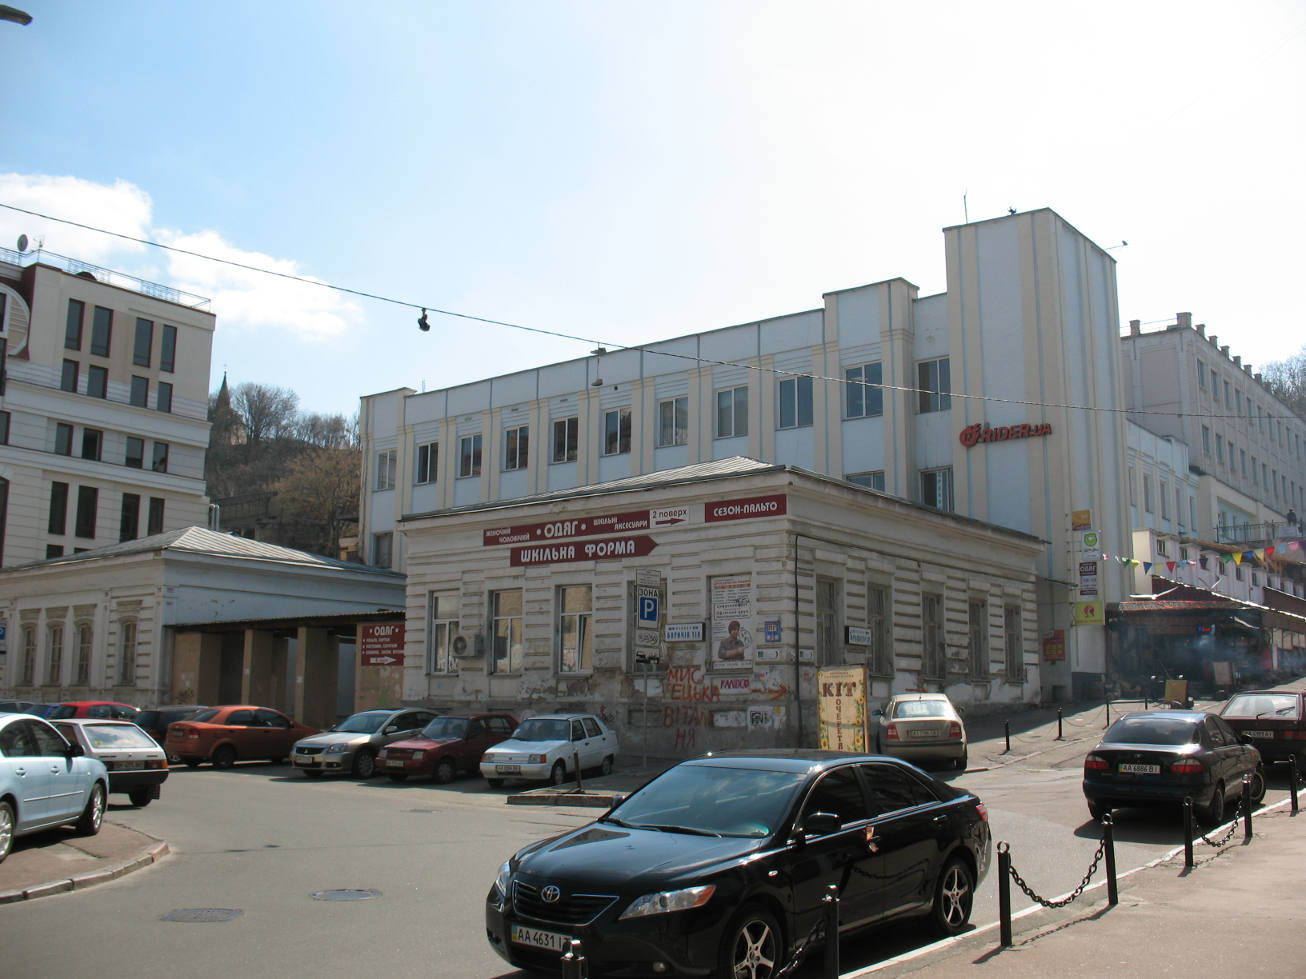
\includegraphics[width=\linewidth]{chast-colebanie-osnov/gora-zamkovaya-valovaya/s_IMG_1490.JPG}
\end{center}

И еще важная фотография. Перед нами Флоровский монастырь, а за ним – опять-таки Киселёвка. Удачно отображена северо-восточная сторона и видно, что кладбищенская стена спускается к монастырю, а вне её продолжается угол горы. Он выходит к современному Житнему рынку, здание которого раньше было рядом, у подножия Щекавицы, вдоль Житнеторжской улицы, где находится автостанция «Подол».

\begin{center}
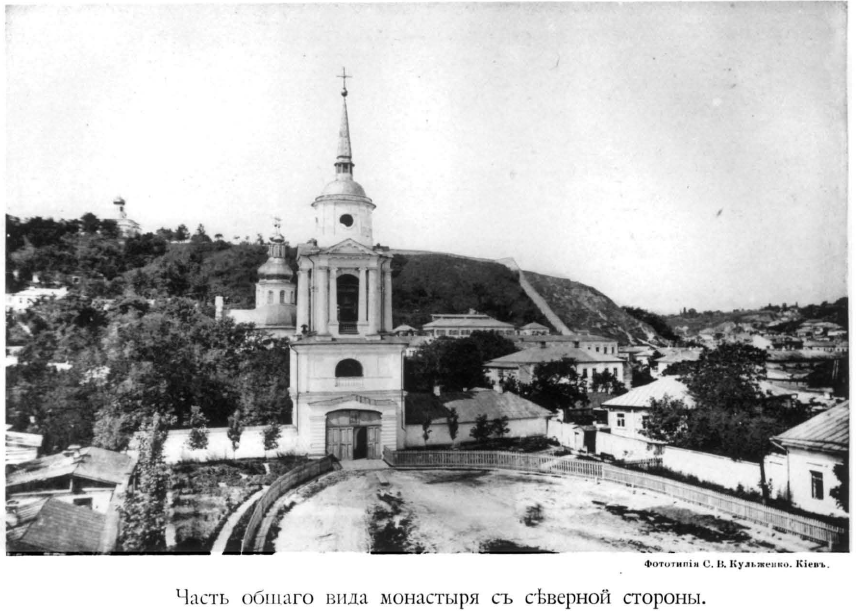
\includegraphics[width=\linewidth]{chast-colebanie-osnov/gora-zamkovaya-valovaya/flor-1894.png}
\end{center}

Поднимемся теперь на соседнюю гору. Уздыхальница, или Здыхальница, расположена по Андреевскому спуску напротив Клинца – с той же стороны, где дом Ричарда Львиное Сердца, и ниже Андреевской церкви.

Уздыхальница уже несколько веков кряду имеет плоскую, искусственно срытую вершину. С одной стороны к горе прилепился дом Ричарда, с другой, внизу – дом №13-А, где жили Булгаковы, и куда писатель поселил в «Белой гвардии» семью Турбиных:

\begin{quotation}
Над двухэтажным домом №13, постройки изумительной (на улицу квартира Турбиных была во втором этаже, а в маленький, покатый, уютный дворик – в первом), в саду, что лепился под крутейшей горой, все ветки на деревьях стали лапчаты и обвисли. Гору замело, засыпало сарайчики во дворе, и стала гигантская сахарная голова. 
\end{quotation}

Если взойти на Уздыхальницу по крутой и гулкой металлической лестнице и подойти к обрыву над восточным склоном, становится очевидным – относительно скромная со стороны Андреевского спуска горка на самом деле высоченная! Это сложно передать фотографией, посему не пытаюсь. Древняя, страшная высота! Снизу она, впрочем, не кажется столь большой. Под Уздыхальницей в сторону улицы Боричев ток, в апреле 2011 торчали обугленные бревна от частного домика, между склоном и трехэтажной кирпичкой. К развалинам вела дорожка из брусчатки.

\begin{center}
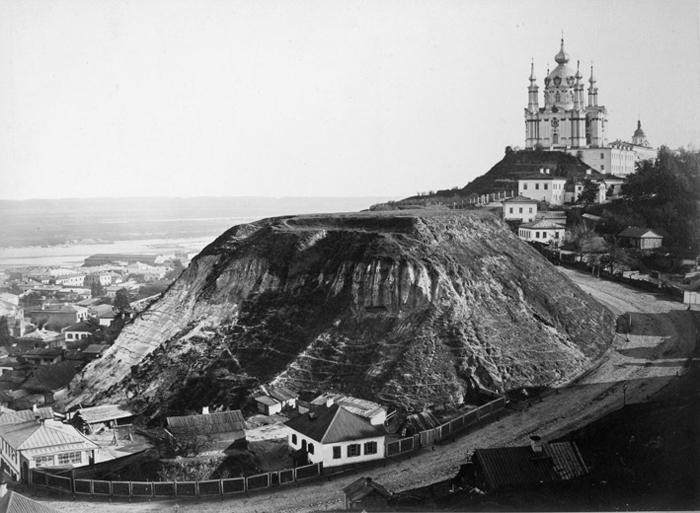
\includegraphics[width=\linewidth]{chast-colebanie-osnov/gora-zamkovaya-valovaya/andreevskiy_spusk.jpg}

\textit{Гора Уздыхальница, вид с Замковой горы, фото 19 века.}
\end{center}

Закревский в «Описании Киева» много усилий приложил к тому, чтобы доказать – Здыхальницей в старину называли одну большую гору, в которой потом прорыли дорогу, ставшую частью Андреевского спуска. Таким образом Здыхальница была разделена на две части, небольшую опять-таки Здыхальницу, и нынешнюю Киселёвку. Закревский упирал на то, что в источниках 17 века нет разделения на Замковую и Уздыхальницу – Боплан и ученый монах Афанасий Кальнофойский упоминали в сочинениях одну только гору. В первом томе «Описания Киева» Закревский в параграфе 67 очень тщательно рассуждает об этом вопросе.

Однако приведу выдержку из документа 16 века, где отдельно, в связи с замком, упомянуты три горы – замковая, Уздыхальница и Клинец. Закревский об этом документе знал, причем видел его в двух версиях, на польском и на «литовско-малороссийском наречии», про этот документ пишет и берет оттуда описание замка – сколько там чего, башен и так далее. О словах про различение гор, входящих в состав замка, Закревский молчит.

В «Описании Киева и Киевскаго замка королевскими люстраторами», 1545 года, из книг Литовской метрики сказано\cite{sbornikmat}:

\begin{quotation}
Гора замковая.

Гора замковая высока досыть и прыкра нижли прилягла близко иньшие горы как же высоки.

От полуночное (северной) стороны за броною воеводиною прилегла гора, на имя Щиковица, с которое видно все посеред замку через стену, бо гора замковая с тое стороны похила на дол, а в середине вышша нижли по краем, а так потребы там впоперек замку тарасу, который бы щитил от горы оное Щиковицы.

А с другое стороны от полудня (южной) за драбскаю брамою только через ров, где может человек каменем зруки докинути, по конец мосту, прилегла гора, на имя Клинец, – ровна з замковою. А другая тамже подалей вышша, на имя Вздыхальнея, але тая остра и может быти унижена копанием.

А еще с третее стороны от заходу солнца, от церкви святого Спаса гора высока также яко замковая.
\end{quotation}

Этот кусок описи замка очень важен. Вначале неско\-лько слов о Клинце. Некоторые сопоставляют Клинец с горой Детинкой (здоровенный горный мыс между улицами Гончарной и Дегтярной). Но ведь в документе ясно сказано, что Клинец – к югу за Драбской брамой замка. Но где была эта «брама», то бишь ворота в башне?

Я сейчас выскажу очень еретическую мысль. Смотрите:

\begin{center}
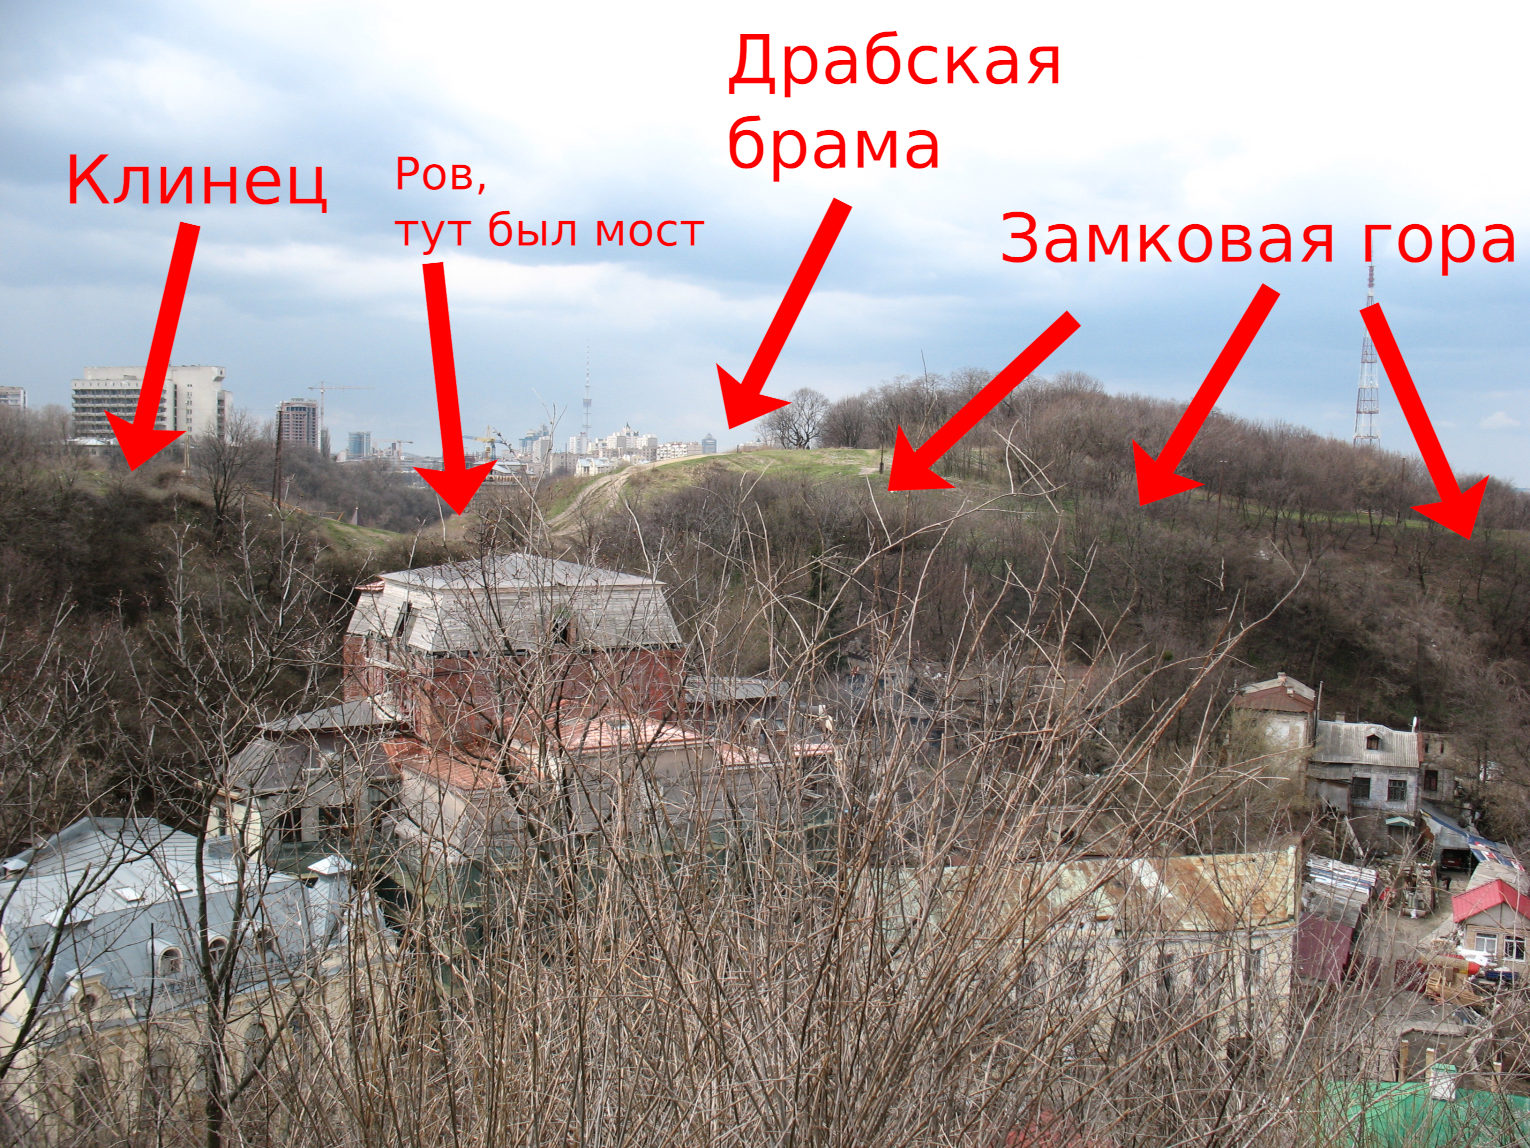
\includegraphics[width=\linewidth]{chast-colebanie-osnov/gora-zamkovaya-valovaya/zamok-scheme.jpg}
\end{center}

%\begin{center}
%\includegraphics[width=\linewidth]{chast-colebanie-osnov/gora-zamkovaya-valovaya/zamok-part01.jpg}
%\end{center}

Ученые полагают дорогу внутри замка по современному Андреевскому спуску, а я – прямо по горе! Почему?

Про северную браму-брону сказано: «От полуночное стороны за броною воеводиною прилегла гора, на имя Щиковица» – то есть северные, Воеводины ворота выходили в сторону Щекавицы. Андреевский спуск туда никоим образом не выходит!

Однако, в северной части Замковой горы до сих пор есть старинная дорога, нисходящая в сторону Щекавицы! Координаты верха дороги – примерно 50°27'46.7"N 30°30'40.5"E. Когда я был там, GPS глючил, а эти числа я привожу по спутниковой карте.

Далее снимок 2011 года. Косые склоны оползней. Сперва усеянное кирпичами путище идет в овраге, ровно, затем начинает петлять, сбрасывая крутизну за счет увеличения расстояния.

\begin{center}
\includegraphics[width=\linewidth]{chast-colebanie-osnov/gora-zamkovaya-valovaya/\myimgprefix IMG_1372.JPG}
\end{center}

В описи обе «броны» занесены в раздел о Замковой горе, а не вне его. Воеводины ворота были на этой старинной северной дороге, наверху или внизу.

Далее мы рассмотрим рисунки Вестерфельда, современника замка. На них в северной стороне крепостной стены изображен проем. Именно там, где начинается сия дорога. Она спускается, если быть точным, по северо-западному склону. 

На обочинах валяются могильные камни и груды кирпича. Им же была выложена дорога, местами еще заметно. Наружность склонов говорит о том, что земля смывалась, с обеих сторон наискось засыпая дорогу. На одном участке она выходит к террасе, а затем продолжается дальше вниз, упираясь в дом по координатам 50°27'48.7"N 30°30'35.0"E в переулке Ладо Кецховели. Не будь там здания, дорога сошла бы точно напротив Щекавицы, начала Олеговской улицы. Со стороны улицы ни дороги, ни террасы не видно, они сокрыты зеленью деревьев.

В конце дороги, на склоне Киселёвки можно найти старинную кирпичную кладку и многочисленные раскопы черных археологов. 

Условия на 2016 год таковы, что выбраться оттуда можно лишь свернув тропой на северо-восток и, пробравшись сквозь крапиву, спрыгнуть с высокого парапета около Житнего рынка, уже на Хоревой. Либо пройти дальше между склоном и задворками Флоровского монастыря, мимо засыпанного давнего погреба, к низу лестницы да к Черной грязи.

Путь к дороге у Воеводских ворот и спуск по ней показан нами в краеведческом фильме «Киевская Амплитуда. Замок».

%\begin{center}
%\includegraphics[width=0.75\linewidth]{chast-colebanie-osnov/gora-zamkovaya-valovaya/\myimgprefix IMG_1374.JPG}
%\end{center}

От Воеводских вернемся ко Драбским воротам. Исходя из описи, Драбские ворота находились: перед рвом, над рвом был мост, а в конце моста – гора Клинец, причем с Замковой до Клинца можно было добросить камнем. В самом деле, там с пригорка на пригорок можно добросить камень! Но как ни старайтесь, вы не добросите камень до виднеющейся с Замковой горы Детинки – далече. 

Вот фотография, сделанная с места, где стояли Драбские ворота. Вид с Киселёвки на Клинец. Можно перекинуть камень на другую сторону?

\begin{center}
\includegraphics[width=\linewidth]{chast-colebanie-osnov/gora-zamkovaya-valovaya/\myimgprefix IMG_1551.JPG}
\end{center}

Можно.

Но вопрос, как дорога продолжалась дальше? Где съезжали с горы? А посмотрите, спускаясь по Андреевскому, на резкий, юго-восточный угол Клинца. Он же явно искусственно обрезан. Думаю, Клинец раньше продолжался, плавно понижаясь примерно к нынешнему пересечению Андреевского спуска и Воздвиженской улицы. Это был покатый, как спина бронтозавра, холм.

Я не знаю, когда его укоротили, привели к нынешним очертаниям. Кстати, лестница на Клинец, по которой все поднимаются на эту гору, полагая её Киселёвкой, в восьмидесятых годах была не сбоку, как сейчас, а шла именно по юго-восточному углу. Даже теперь там остается тропка.

По предыдущей фотографии не видно глубины рва между Клинцом и Киселёвкой. Поможет другое изображение, где какие-то люди поднимаются на Киселёвку, а я фотографирую, стоя внизу рва:

\begin{center}
\includegraphics[width=\linewidth]{chast-colebanie-osnov/gora-zamkovaya-valovaya/\myimgprefix IMG_1547.JPG}
\end{center}

А что значит название «Драбские» ворота? Возможно, от «драбына» – лестница. Однако в войске Великого княжества Литовского были «драбы» – говоря в общем, вид пехоты. Иногда использовались как стражники.

Еще сказано про соседнюю гору: «А другая тамже подалей вышша, на имя Вздыхальнея». Так и есть – Уздыхальница расположена там же, но подальше и выше.

Но по Закревскому, башни-ворота стояли не на горе, а на прорытом через гору спуске, теперешнем Андреевском, который служил дорогой внутри замка, сам же замок располагался на территории всей рассеченной горы – обеих нынешних и Киселёвки, и Уздыхальницы.

Голландец Абрахам ван Вестерфельд (Abraham Evertsz van Westerveld, 1620/21-1692), придворный художник литовского гетмана Януша Радзивилла, того самого, именем коего названа известная летопись (владел ею), прибыл вместе с последним в Киев летом 1651 года, когда Польша с Хмельницким тягалась. Радзивилл помогал Польше.

Вестерфельд создал целый альбом рисунков с видами города. Они дошли до нас в копиях конца 18 века, изданных дореволюционной книгой-исследованием «Рисунки Киева 1651 года по копиям их конца XVIII века» Смирнова.

В прочих, в том числе современных, книгах время от времени появляются «рисунки Вестерфельда», причем один и тот же вид порой представлен несколькими вариантами. Ежели рассуждать о них подробно, понадобится целая книга. Примем как есть – известны копии рисунков Вестерфельда. Ими и будем пользоваться, называя оные дальше просто «рисунками».

В вопросе о замке особо важны два рисунка Вестерфельда, с видом на Киев со стороны северо-востока. Отдельная картинка, кочующая из книги в книгу под названием «Киевский замок», срисована со второго из них.

Работы Вестерфельда принимаются историками за единственные уцелевшее до наших дней документальные изображения Киева того времени. Но забывают учесть некоторые вещи. 

Мы не знаем, сколь точен был Вестерфельд в подробностях. Не знаем и насколько точны были копировальщики. На иллюстрациях в книгах мы видим \textbf{разные} варианты – сие касается соотношения высоты и ширины, пологости склонов, наличия на них растительности, разных бугорков, наконец зданий. Сейчас невозможно сказать, что показано правдиво, а что вымышлено. Сравнить не с чем – нет других изображений Киева тех же лет.

Однако, если подлинники Вестерфельда использовались Радзивиллом как планы местности при разработке военных операций, то художник был предельно точен. Скрупулезно показаны, например, бойницы в стенах. Четко вырисованы отдельные здания, рощи.

%Все полноразмерные варианты «вида на Киев» выкладываю \href{http://semiletov.org/kiev/ext/verterfeld-zamok.zip}{по этому адресу}. Здесь буду пользоваться разными вариантами, чтобы показать вам отличия и сходство, и не брать на себя роль судьи в определении точности приближения к подлиннику.

%Буду пользоваться разными вариантами, чтобы показать вам отличия и сходство, и не брать на себя роль судьи в определении точности приближения к подлиннику.

Основополагающими и наиболее точными считаю два следующих рисунка из книги Смирнова. Они составляют вместе панораму вида на правый берег. Помещу сначала вместе, без отметок. 

\newpage
\vspace*{\fill}
\begin{center}
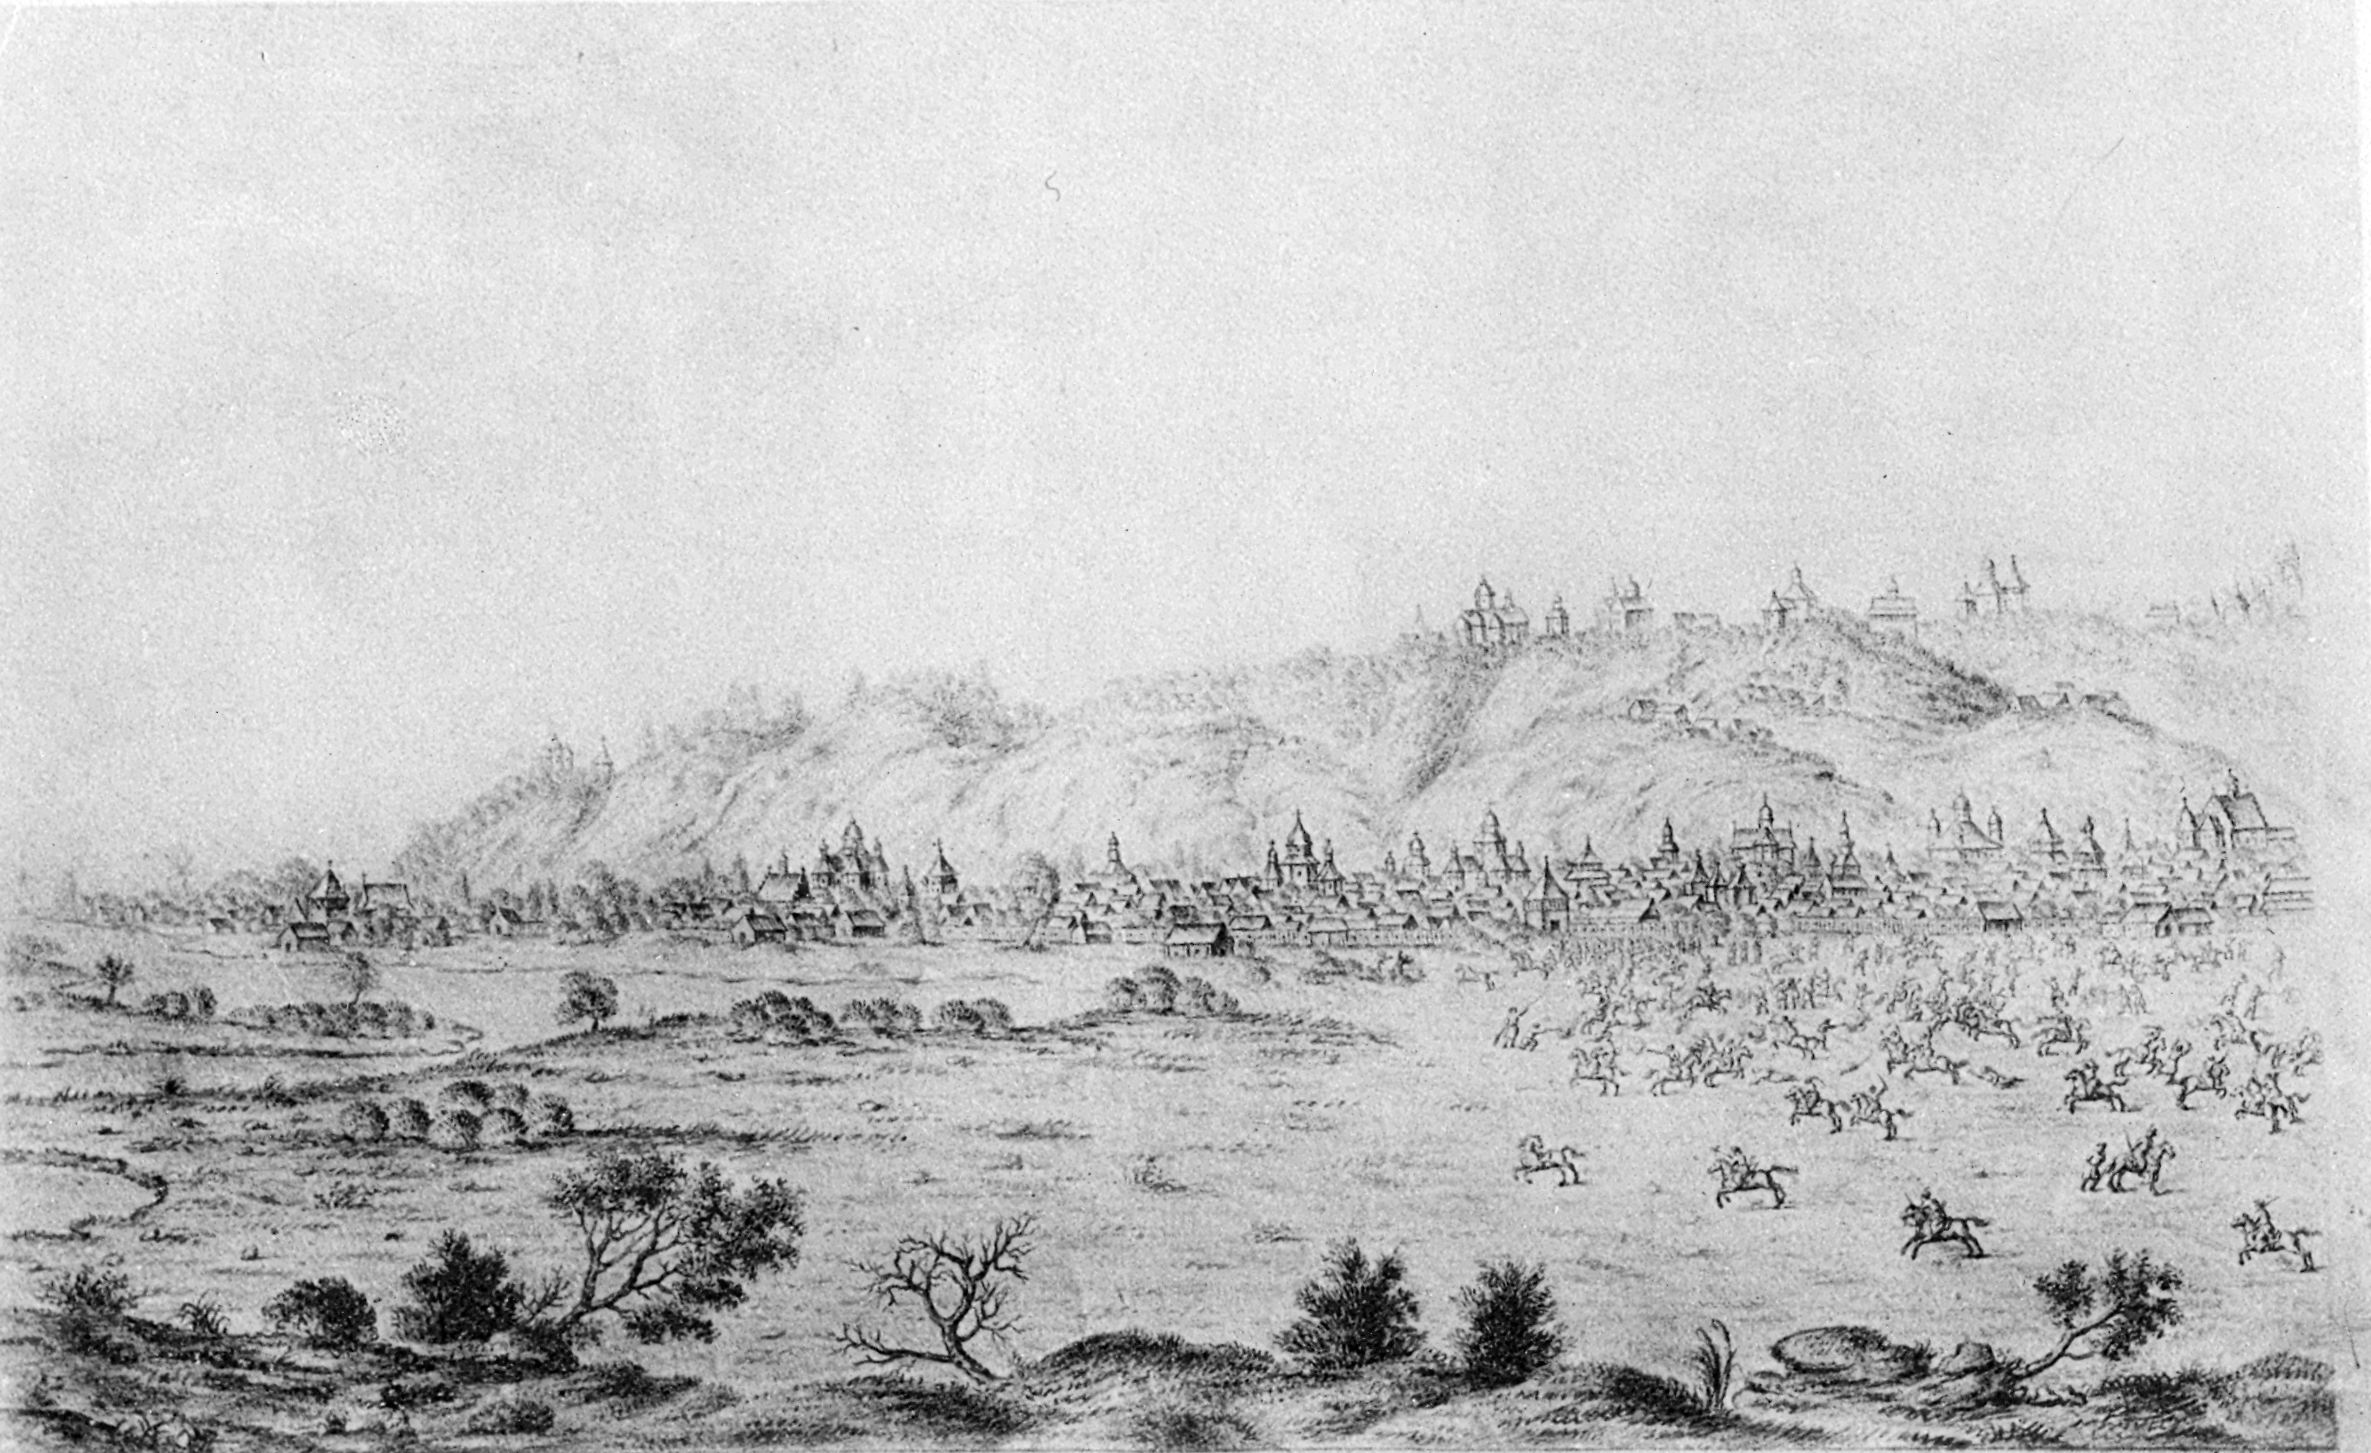
\includegraphics[width=\linewidth]{chast-colebanie-osnov/gora-zamkovaya-valovaya/tabl03-1.jpg}
\end{center}

\begin{center}
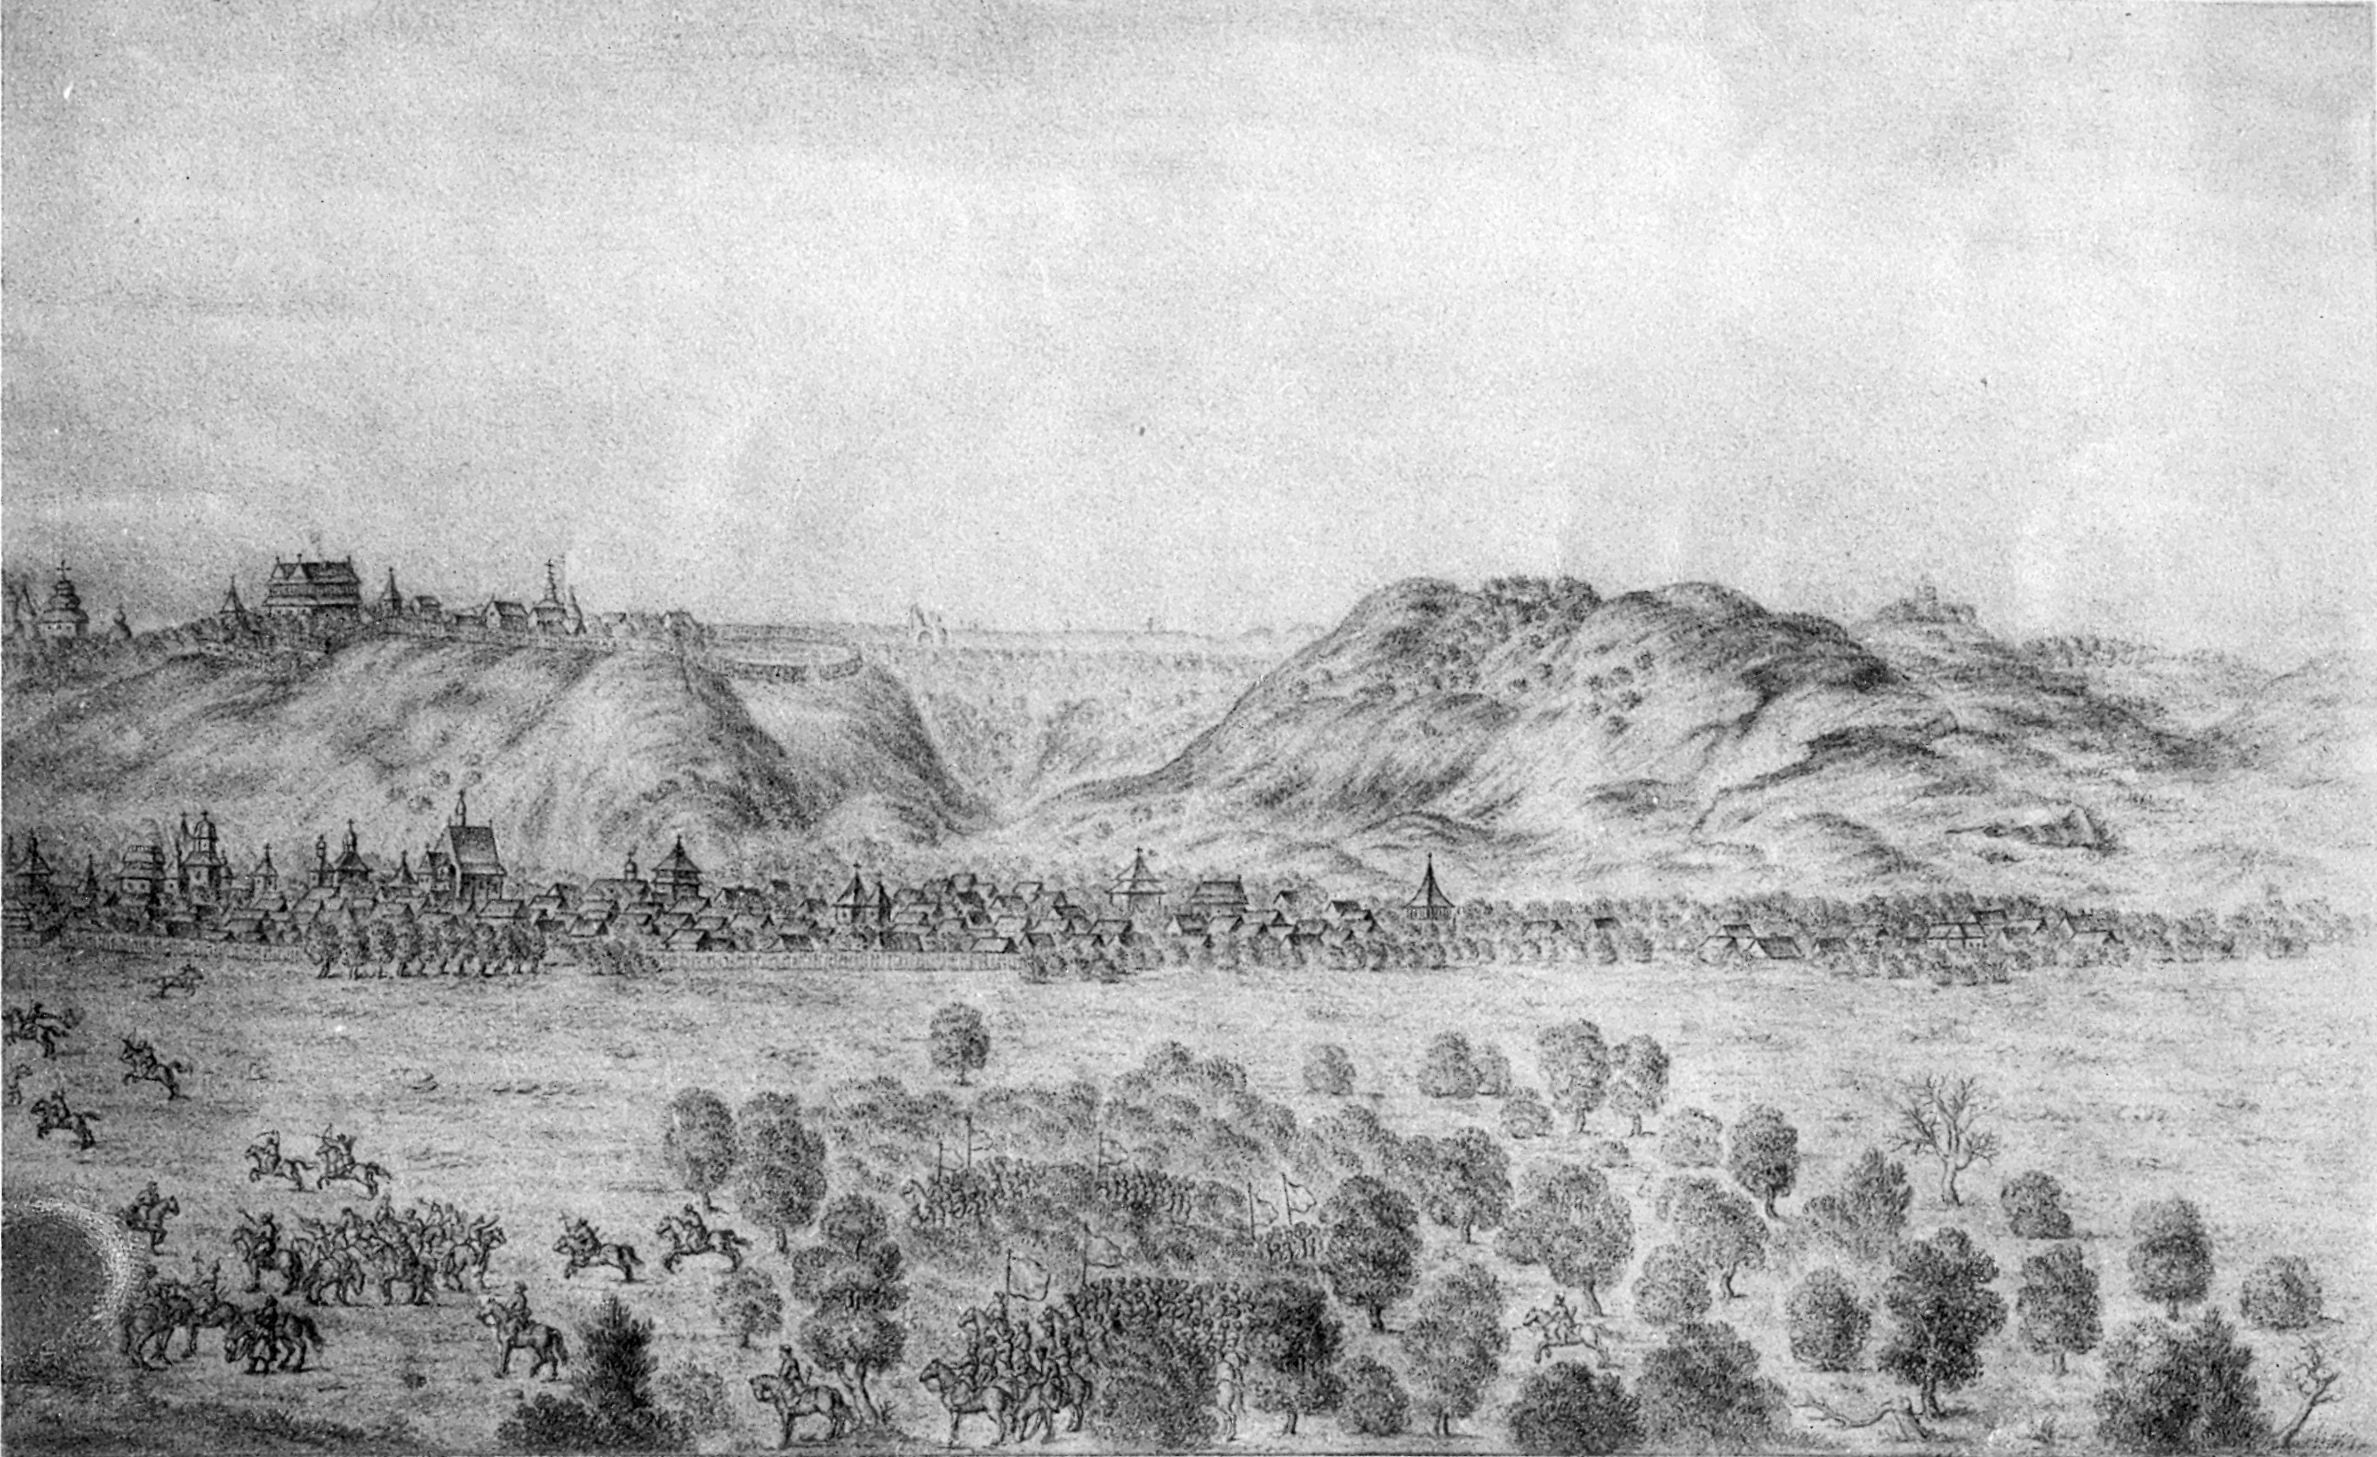
\includegraphics[width=\linewidth]{chast-colebanie-osnov/gora-zamkovaya-valovaya/tabl03-2.jpg}
\end{center}
\vspace*{\fill}
\newpage

\begin{center}
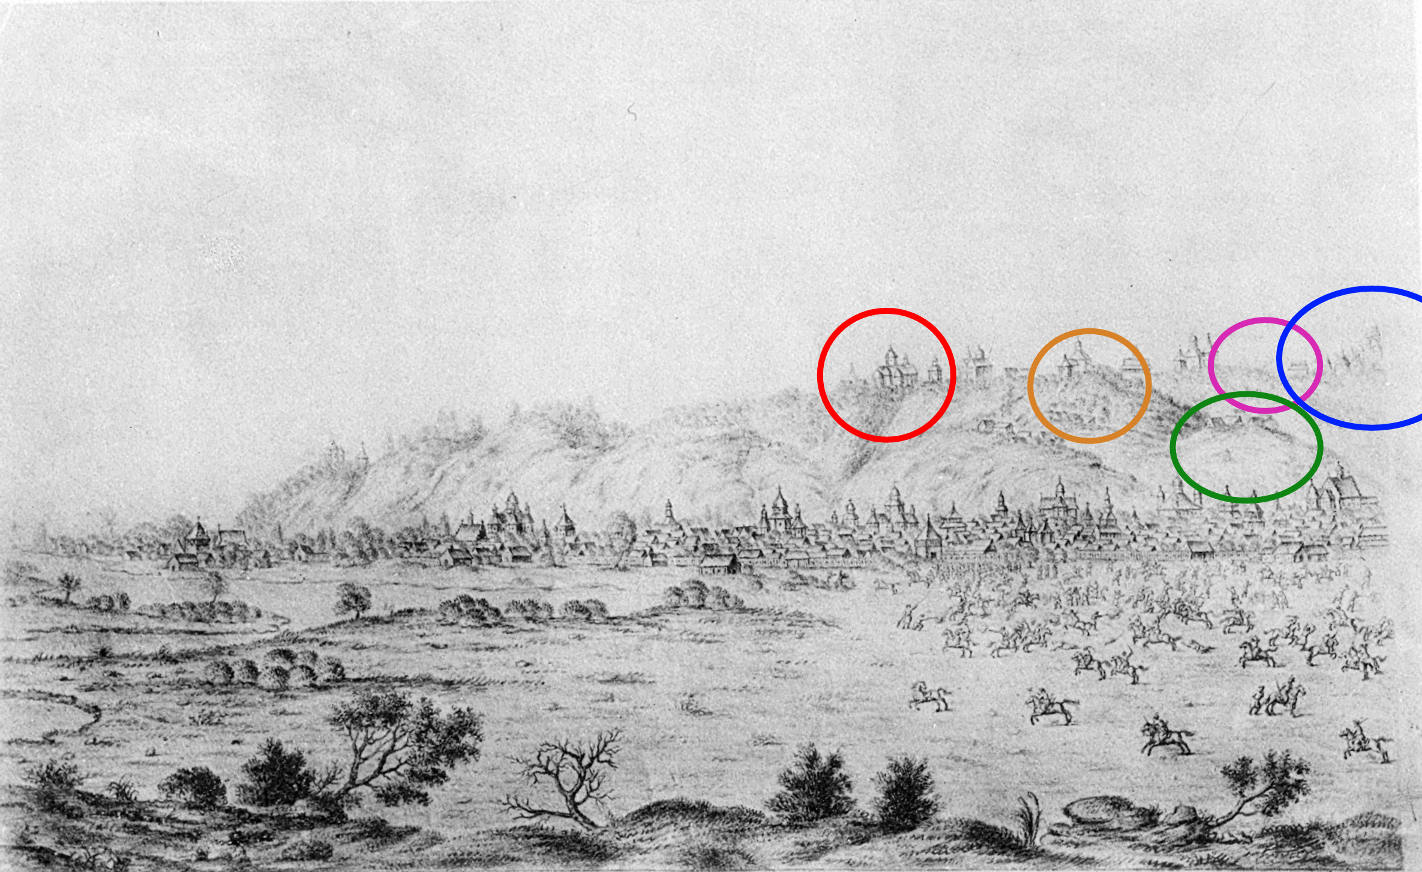
\includegraphics[width=\linewidth]{chast-colebanie-osnov/gora-zamkovaya-valovaya/tabl03-1-marked.jpg}
\end{center}

Красным кружком я обозначил Михайловский монастырь над оврагом Боричева. Оранжевый – пригорок, где ныне стоит Андреевская церковь. Зеленый – Уздыхальница. Синий – на заднем плане виднеется София. Малиновый – Клинец.

Художник показал не наблюдаемое из одной точки, но запечатлел взаимное расположение гор. Если одна при обзоре перекрывала другую, Вестерфельд делал перекрываемую чуть выше, а перекрывающую – ниже, чтобы отобразить обе. Если же один отрог находился за другим, дальний отрог выносился несколько в сторону.

Киев был срисован до того, как войска Радзивилла два дня жгли город. Церкви в целости, а известно, что из крупных сооружений на Подоле после того пожара уцелел только каменный монастырь Доминиканцев. Значит, рисунки сделаны до конца июля 1651 года, ведь уже в августе силы Хмельницкого зажали Радзивилла в городе, а к 1 сентября литовский гетман оставил Киев, ценой тяжелых потерь.

Обратите внимание на равнину перед Подолом. Слева видно излучину реки. Это наверное Днепр. Угол излучины – эдак напротив Почтовой площади. Правее – поле со всадниками, значит, реки там нет. А где же пристань? Допустим, тогда пристань была в другом месте. Но известные по плану 1695 года Почайна-2, Днепр, острова между ними, мосты?

Подол огражден от поля стеной с бойницами. Знаменитый «палисад». Прикинем, где по современному Подолу проходила эта линия. Умозрительно у меня не выходит. Могут ли помочь в качестве ориентиров какие-нибудь церкви? 

Да, Борисоглебская, что простояла с 1692 года по двадцатый век в месте, где ныне дом по адресу Борисоглебская, 10 (250 метров от набережной). Прежде 1692-го, по словам Похилевича в книге «Монастыри и церкви Киева», там был одноименный деревянный храм. Допускаю, он существовал и в 1651-м, поэтому должен быть отражен и на рисунке, и на плане. Также нам подсобит церковь Святого Духа, ныне это Сковороды, 2. Всё это есть на куске перерисовки плана Ушакова: 

\begin{center}
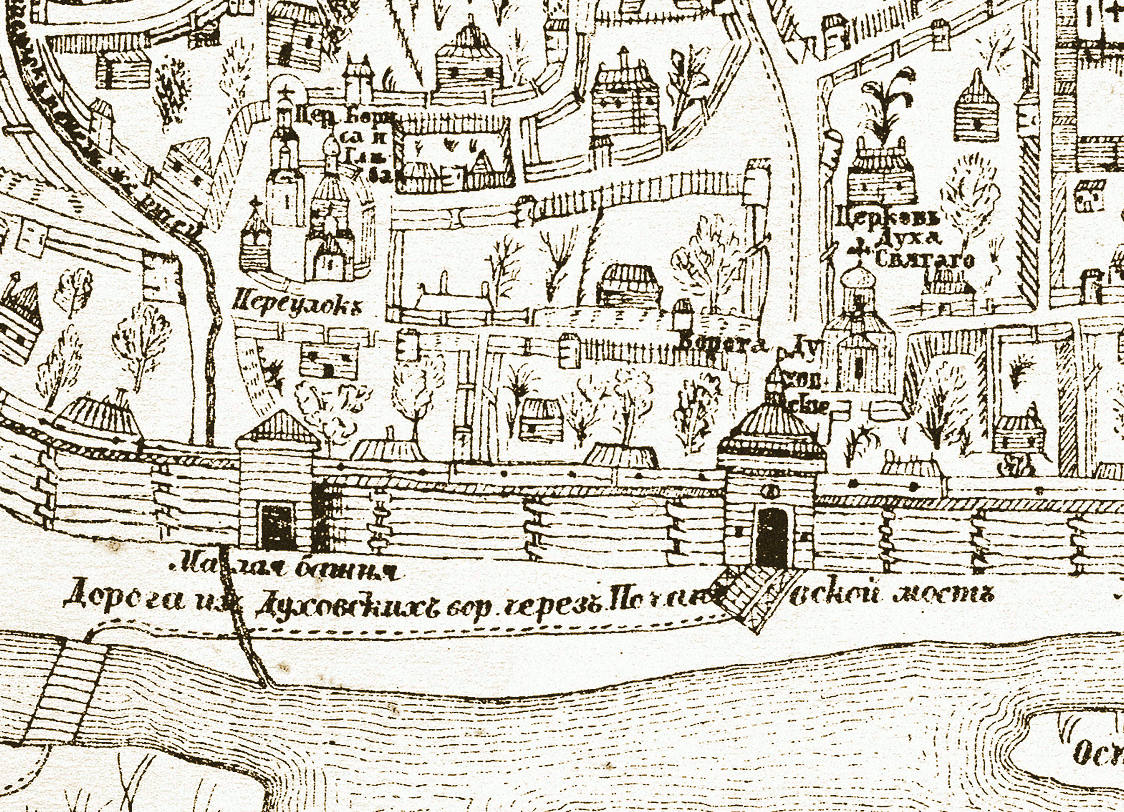
\includegraphics[width=\linewidth]{chast-colebanie-osnov/gora-zamkovaya-valovaya/boris.jpg}
\end{center}

Как видим, от подольской восточной ограды (внизу) обе церкви отделены расстоянием примерно в один двор. Внимательный читатель отметит также, что на плане нет каменной церкви Ильи (Почайнинская, 2), возведенной в 1692 году сотником Гудимой. Она должна быть правее Борисоглебской и ниже Святого духа.

Но для определения населенных пределов Подола нам довольно и этих двух. Можно сказать, что Подол  в 1695 году был населен приблизительно по нынешнюю улицу Волошскую, остальное же место к реке занимало поле. Это поле имеет незавидный размер по вертикали на плане Ушакова, и громадно на рисунке 1651 года, что вероятно согласуется с современным пространством от набережной до Волошской.

Поскольку на рисунке перед нами не видно Днепра и Почайны-2, показанные там на плане 1695 года, можно сделать один из выводов:

1. Поле между рекой и подольской стеной на плане Ушакова отражено с ошибочным размером по вертикали.

2. В 1651 году там была суша, а к 1695-му ее прорыли русла Днепра и Почайны-2. 

%Ни на одном из двух рисунков 1651 года, этих половинок целого, я не вижу Почайны-2 как рукава Днепра, не вижу больших островов с мостами между ними. Равнина! 

%На уровне Михайловского монастыря, в удольи, заметно идущее слева русло, в коем я предполагаю излучину Днепра, но правее русло прерывают много всадников и пеших, значит, согласно рисунку, между стеной с бойницами и полем ничего существенного не протекало.

Обсудим теперь вторую страницу панорамы.

\begin{center}
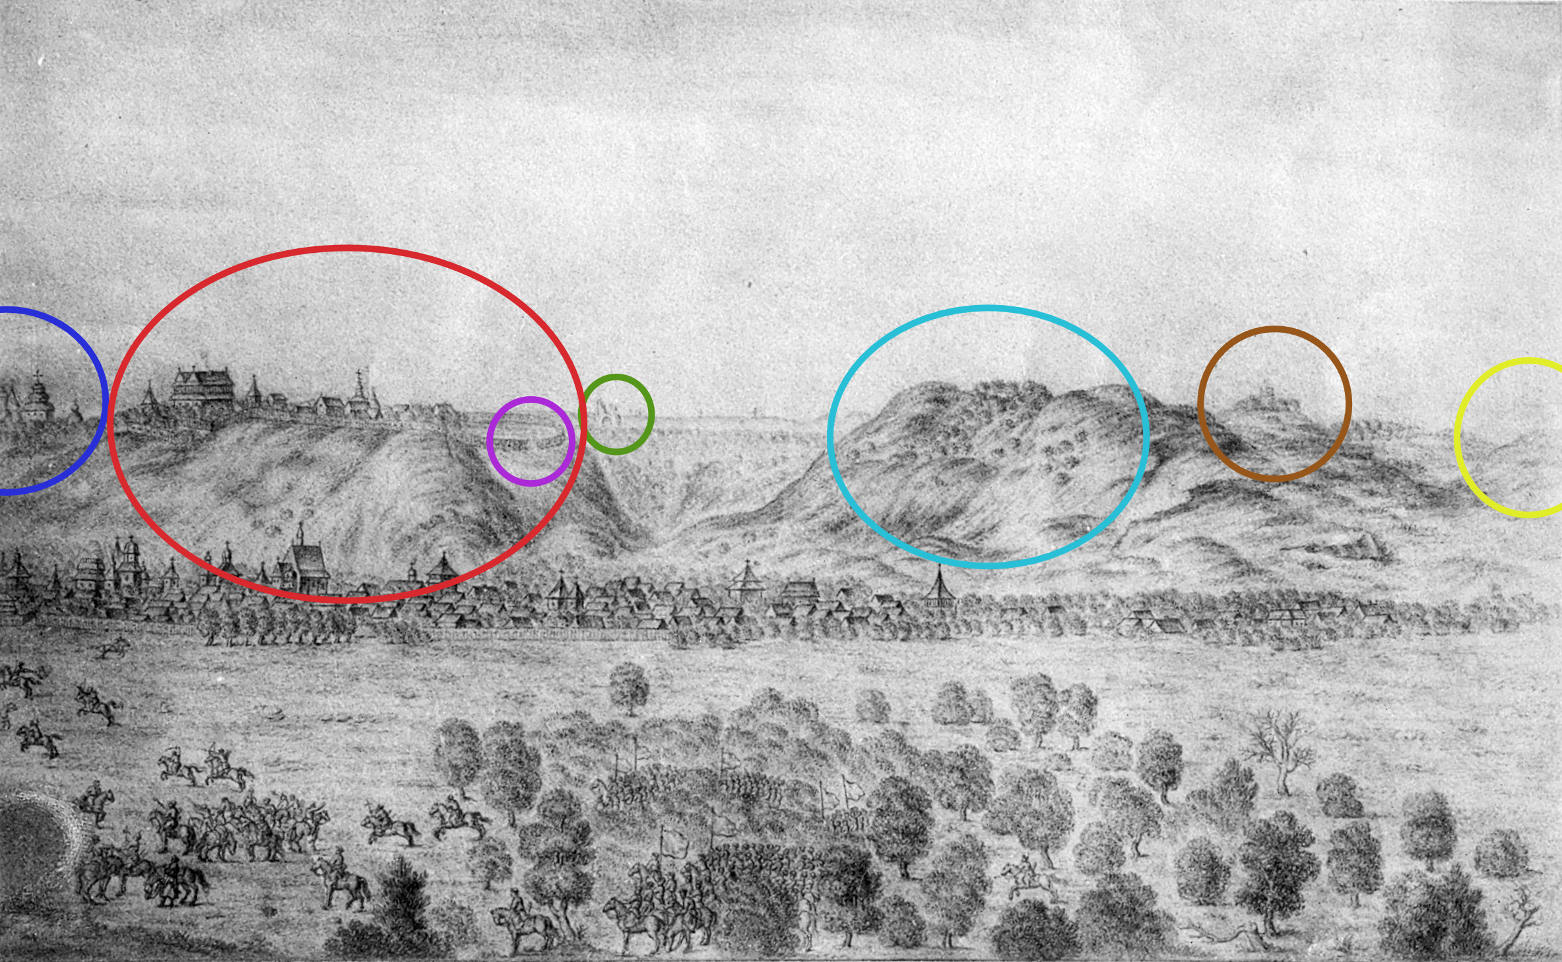
\includegraphics[width=\linewidth]{chast-colebanie-osnov/gora-zamkovaya-valovaya/tabl03-2-marked.jpg}
\end{center}

Слева, синий кружок – между Замковой и Клинцом выглядывает София. Красный – Замковая гора. Фиолетовый – проем в ограде замка. Зеленый – разрушенные ворота в Пробитом валу на Кудрявце. Бирюзовый – гора Щекавица. Коричневый – «старая Юрковица», нынешний отрог Щекавицы с кладбищем старообрядцев (на рисунке там изображены, вероятно, остатки какой-то крепости). Желтый – «новая Юрковица», прежняя Лысая гора.

Постройки замка стоят на горе, где ныне остатки кладбища Флоровского монастыря. Видим голую траву, никаких деревьев или кустов, не то что ныне. Двор замка обнесен невысокой стеной с бойницами. Склоны холмов, образующих долину между Киселёвкой и Щекавицей, показаны в измененной перспективе, являя все отроги. 

Проем в стене находится на северо-западном склоне Киселёвки, против Щекавицы. Там же, как мы знаем по описанию, были Воеводские ворота. Поскольку иных проемов в стене не видно, значит, ворота эти могли находиться только там.

Я не знаю состояние Воеводских ворот при Вестерфельде. Возможно, башню над ними разрушили несколькими годами ранее, когда войска Хмельницкого брали город и захватили замок. По 2020 год, на том же северо-западном склоне существует единственный оттуда, старинный спуск.

Проем отчетливо просматривается и на других копиях рисунка Вестерфельда, чего не скажешь о вообще каких-либо очевидных дорогах от замка вниз. Кроме того, в 1651 году замок сосредоточен на Киселёвке, Уздыхальница же вне его ограды, торчат угловатые скаты крыш каких-то домов.

Павел Алеппский (Paul Aleppo), архидиакон Алеппо, родной сын патриарха Макария III, сопровождая оного, побывал в Киеве в 1653 году. Впечатления о поездке по нашим землям он изложил в книге «Путешествие Антиохийского патриарха Макария»\cite{alepp02}. 

Павел пишет, что «древний город Киев», осажденный врагом, после долгой войны обратился в руины, жизнь же сползла в долину, на берега реки Непрос. Путь туда, в новый город, лежит через одни ворота замка, а затем надлежит выехать сквозь другие, после чего вы спускаетесь длинным узким проходом, чрезвычайно неровным, ширина коего с трудом достаточна для лошади с повозкой. Крепость же, сооруженная недавно, находится на вершине холма, откуда открывается вид на весь лежащий внизу город\footnote{Переведено мною с английского перевода с арабского: «The way to is by the entrance of once gate of the castle, and out through the other; after which you descend by a long narrow passage exceedingly rough, and of hardly sufficient width for a horse and a carriage to the modern town: for the fort, which they have now recently constructed on the top of the hill, whence you look down over the whole city below».}.

Кажется, Алеппский ясно говорит – крепость (замок) стоит на вершине холма, а чтобы спуститься в нижний город, надо въехать в одни ворота замка и выехать в другие. Где ворота замка? Если замок на холме, то и ворота там же. И описание прохода от ворот весьма подходит к сохранившейся старинной дороге.

В книге «Descriptio Sarmatiarum» доктора медицины и краковского каноника, географа, историка Мацея Миховского (1457-1523) про Киев говорится, что есть возле него гора, по которой купцы перебираются с трудом. Ежели что при тяжком подъеме ломается в повозке, то весь товар идет в пользу казны\footnote{Ad Chiovam monticulus quidem est, per quem mercatoribus via aliquanto difficiliore transeundum est; in cuiuis ascensu si forte currus aliqua pars frangatur, res quae in curru portabantur, forte vindicantur.}. 

Про это Миховскому поведал Альберт Гастольд, виленский палатин и наместник львовский. Барон Зигмунд Херберштейн (Sigmund Freiherr von Herberstein), бывший на Руси в годах 1517 и 1526, минуя впрочем Киев, в своей книге «Записки о Московии (Rerum Moscoviticarum commentari) безо всякого смущения помещает слова Миховского уже от своего имени.

Переться на гору купцы могли только в одном случае – через Замковую. И не вдоль, не под нею, а непосредственно по ней.

Почти столетие спустя после известия Миховского, в Киеве еще действовал закон, предписывающий отбирать товары с поломавшихся возов. Пошлина с купцов взималась тогда по количеству возов. И хитрецы стали грузить на телеги побольше, чтобы сократить количество повозок и размер налога. Но чрезмерно отягощенные телеги часто ломались. В грамоте литовского князя Александра от 14 мая 1499 года сказано:

\begin{quote}
Которые купцы, коли едут с Киева, и возы свои товаром тяжко накладывают для мыта, ижбы возов меньшей было. И в которого купца воз поломится с товаром, на одну сторону по Золотыи ворота, а на другую сторону по Почайну реку, ино тот воз с товаром биривали на воеводу киевского;
\end{quote}

Биривали – то бишь отбирали.

Думая над рассуждениями Закревского про большую общую Здыхальницу, я прихожу к мысли, что между Замковой и Уздыхальницей всё же лежал овраг, а горы таки были разделены. И потом этот овраг прокопали да расширили для удобного проезда. Сами очертания Клинца, Киселёвки и Уздыхальницы указывают на то, что к ним явно было применены земляные работы.

Сведения об этом сохранились в источниках. «Хроника о разных речах»\cite[стр. 85]{sbornikletug} говорит – в скобках поясняю некоторые слова:

\begin{quotation}
Року 1617 (в 1616 по другому списку) при великом короли Жикгимонте, а при пану воеводе Киевском, Станиславу Жолковском, старанием и накладом (деньгами) панов мещан Киевском: на тот час пана войта Федора Ходыки и пана бурмистра Матфея Мачохи и всего посполства места (города) Киевского, скопали гору Уздыхальницу, которая стоит пред замком Киевским, и еще знать; а скопано еи на полшеста сажня добрых у звышки и нашли там печерку сажней трех у гору глубоко а в ширь сажня; и нашли в неи горщик ни щим (пустой) а большей ничого, и написано на стене имя: «Павел»; знать же то колись, был пустельник (Отшельник).
\end{quotation}

«Полшеста сажней», или 5,5 сажней – сколько это в метрах? А сложно сказать. Не знаю, чему равнялась сажень в то время в тех документах. Было множество сажней – от полутора до более двух метров. Но ежели брать наименьшее, можно считать, что Уздыхальницу понизили эдак на высоту двухэтажного дома с плоской крышей. Как мы помним из описи Замка, Уздыхальница была «вышша» и могла быть уменьшена «копанием». Вот и уменьшили.

%Когда в 1649 году казаки под предводительством Хмельницкого громили в Киеве поляков, то разрушали всё польское – костелы, кладбища. На улицах для потехи выставляли гробы со останками поляков. Вероятно, уничтожили и замок – упоминаний о нем в истории больше нет. 

Неясно, когда сгинул замок на Киселёвке. Рисунки Вестерфельда кажутся последним свидетельством про него.

Эдак по 1830 год на Замковой горе киевляне разводили огороды и баштаны, да летом устраивали кулачные бои. После передачи горы Флоровскому монастырю в 1854-м, три года спустя там появилось кладбище и сад. Сад поначалу был возле одноэтажного домика, построенного у кладбищенского Троицкого храма Флоровского монастыря. Погост с садом обнесли оградой – стеной, которая обошлась в копеечку по причине плохих условий строительства, уж больно склоны крутые.

Напротив Замковой, к северо-западу – огромная гора Щекавица.

Но прежде чем отправиться туда, обратим внимание на возвышенность, что виднеется на рисунке Вестерфельда между Замковой и Щекавицей, в глубине. Ранее я отметил там разрушенные ворота в Пробитом валу. В некоторых других копиях рисунка, на углубленном склоне холма, по верху идут заросли. А здесь другое – крепостная стена или вал. И в нем развалины неких ворот.

Увеличенный кусок рисунка:

\begin{center}
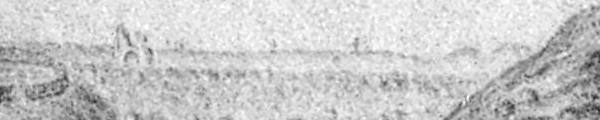
\includegraphics[width=\linewidth]{chast-colebanie-osnov/gora-zamkovaya-valovaya/val-big.jpg}
\end{center}

Развалины ворот, обращенные проемом на северо-восток, сами несколько возвышаются над валом. Правая сторона его уже теряет очертания. Предположу, что ворота заделаны, поскольку от них не ведет дорога. Если ее не упустил из виду художник.

Что за местность?

Сейчас наверху Львовская (прежде Сенная) площадь, и вал длится, судя по рисунку, вдоль улиц Артёма и Большой Житомирской, вероятно по Кияновскому переулку да улице Кудрявской, нависая восточной частью над Гончарами и Кожемяками. Это не Ярославов вал – ведь тот, по общепринятым представлениям, шел от Золотых ворот к той же Львовской площади.

Итак, вал с воротами. Они вероятно выходят в сторону нынешнего Вознесенского спуска (Смирнова-Ласточ\-кина), что нисходит горой Воловней (на поздний картах Воловьей). По внутреннюю сторону вала, следовательно, была некая оберегаемая валом местность, где жили люди – от указанных улиц на юго-запад. Мы видим, что вал идет на северо-запад, вправо, чуть не до Лукьяновки! Границ вала на рисунке нет, не помещаются.

Это меняет сложившиеся представления о небольшом «верхнем городе», который вроде был ограничен с одной стороны Ярославовым валом (по ходу одноименной улицы), Львовской площадью и северо-восточными склонами холмов Старокиевской горы. Вал до Лукьяновки не будет просто сам по себе, верно?

Любой вал разделяет местность на пространство внутреннее (охраняемое) и внешнее. Во внешнее в нашем случае попадают гора Воловня, Кудрявец, Гончары, Кожемяки. Во внутреннее, огражденное – а прикиньте сами. Это могла быть вся местность аж до площади Победы, до цирка. Улицы Чкалова (Гончара), Бульварно-Кудрявская (Воровского), Тургеневская, Володарского (Златоустовская), Дмитриевская.

А ведь мимо Златоустовской поныне, еще от Белорусской, протекает в коллекторе ручей с явно давним славянским названием Скоморох. Так могли наречь только до властвования над Киевом Литвы с Польшей. А ручьи именовались лишь протекая по населенной местности. Хотя более важным кажется мне, что жители домов окрест ручья кликали его речкой Лыбедью, я про это уже говорил. Предполагаю, что Лыбедь, состоящая из «Скомороха» и привычного нам отрезка Лыбеди от Вокзала до устья чуть южнее Зверинца служила западной и южной границей града Киева в пределах правого берега Днепра. 

На плане-реконструкции Закревского «Киев от 1400 до 1600 года» вал с рисунка Вестерфельда присутствует частично – восточная его часть обозначена «Пробитый вал», а дальше у Закревского он заканчивается на Львовской площади, и Ярославов вал служит его продолжением до Золотых ворот. 

Однако на рисунке Вестерфельда мы видим картину противоположную – вал, названный Пробитым у Закревского, не завершается там вовсе, а следует к западу. На старых картах, начиная с плана Ушакова, вал сей прослеживается по верхам Кудрявца, с годами меняя очертания и потихоньку исчезая.

Эрих Ляссота, бывший в Киеве в 1594 году и описавший свое посещение в дневнике (Tagebuch des Erich Lassota von Steblan. Helli. 1866) сообщает о некоем огромном валу:

\begin{quotation}
Киев был очень укреплен на обширном пространстве и украшен великолепными церквами и зданиями, общественными и частными, как можно судить об этом по древним развалинам, равно и по валу, охватывающему город, и простирающемуся, говорят, на девять миль в окружности.
\end{quotation}

Неясно, какая миля используется. Было много видов миль. Но девять – никак не менее девяти километров. Полукруглый вал вокруг Киева показан на польских картах 17 века, однако они весьма условны.

Профессор Петров в «Историко-топографических оче\-рках древнего Киева»\cite{petrov01} имел мнение о Пробитом вале, противоположное моему – что защищаемая валом местность находилась в сторону Подола, то есть внутри огороженной местности оказывались гора Воловня, Кудрявец, Гончары и Кожемяки, Житний рынок и так далее к реке. 

Но вал шел по краю горы, гораздо выше окрестностей Подола. Что это значит? Точку зрения Петрова можно уподобить возведению вала жителями котлована вокруг своего котлована, по ободку. Себе на погибель! Со стороны Подола, Пробитый вал – надстройка над склоном, естественным защитным рубежом. Нападающие сверху, с юго-запада, будут в гораздо более выгодных условиях, чем обороняющие снизу, с северо-востока, Подола. Нет, Пробитый вал построен в таком месте, где подразумевается нападение только со стороны Подола, а не с обратной, как полагал Петров.
 
Как же назывались ворота в валу, изображенные Вестерфельдом? Попытка ответить на этот вопрос приведет нас ко множеству рассуждений о киевских воротах, к чему я покамест не готов. Ворота можно соотнести с окрестностями Львовской площади. Ученые уже несколько веков говорят, что там стояли сначала летописные Жидовские ворота, а затем позднейшие Львовские или Житомирские. Утверждение насчет первых нельзя проверить. Я бы не спешил сопоставить развалины ворот и со Львовскими.

Кстати, в 1874 году в районе Львовской площади (в усадьбе, третьей по счету от нее) при рытьи траншеи нашли клад из 4000 римских монет – денарии Адриана, Антонина Пия и Марка Аврелия. Сокровище разобрали по рукам землекопы.

От площади вниз, на север, до перекрестка с Глубочицкой улицей, по горе Воловне сходит Вознесенский спуск. В 19 веке место перекрестка именовалось Кожемяцкой площадью. К юго-западу оттуда, в удолье между горами Замковой, частью Кудрявца и Детинкой лежит урочище Гончары и Кожемяки. Там же проходят давние улицы – Кожемяцкая, Дегтярная (тоже указывает, кто здесь жил), Гончарная, Воздвиженская. До конца 20 века здесь сохранялась старая застройка. В этой просторной балке, теперь заставленной похожими на торты домами, протекал приток Глубочицы – Киянка, ныне взятый в коллектор. Из плана Ушакова ясно, что в 1695 году кожемяцкая слобода находилась в другом месте, у Щекавицы, примерно подле начала Олеговской улицы.

Холм по ходу Вознесенского спуска называется горой Воловней. К востоку от него лежит мыс, гора Детинка. А к западу, через Вознесенский яр (в нем лежит Петровская улица) – гора Кудрявец, она по четной стороне Глубочицкой улицы. Кудрявцем называли прежде и речку Глубочицу. Земельные документы 17 века овраг, где она протекала между Щекавицей и противоположной горой Кудрявцем, именовали «долина Кудравец». Кудрявец это растение лебеда душистая (chenopodium botrys). Вспомним подобные растительные названия в Киеве – Репяхов Яр, речка Коноплянка, Хвощеватая долина.

На возвышенном мысу горы Воловни по четной стороне улицы, ниже художественной академии расположена больница Академии наук с живописным двориком, где приютилась статуя Амура. 

Этот мыс северо-восточной стороной выходит в Кожемяки, северной обращен к дороге, вероятно именно на нем, у обрыва\footnote{50°27'40.09"N 30°30'18.6"E} над поворотом, в 1878 году местные кладоискатели раскопали окруженный рвами, обсаженный липами, поросший травой курган, оказавшийся на проверку древними развалинами. Они состояли из мусора, обломков кирпича, щебня, плит из красного шифера – пирофиллитового сланца. Кладоискатели поняли, что это не языческий курган, потеряли интерес, и засыпали развороченное.

Сведения о раскопках дошли до Церковно-археологи\-ческого общества при Киевской духовной Академии. Подробности раскопок, проведенных уже обществом, описал Петр Лашкарев в работе 1879 года «Развалины церкви св. Симеона и Копырев конец древнего Киева». Он сопоставил находку с церковью святого Симеона, а местность с Копыревым концом. Лашкарев пишет, что кто-то из местных назвал окрестности церкви на Кудрявце «Ольговой могилой».

Что же отыскали во время «официальных» раскопок? Следы пожара. Остатки фундамента и стен, подпорных столбов. Черепки, разрозненные человеческие кости, часть скелета, ржавый железный нож, куски олова, медные кусок колокола и крючок. Никаких церковных вещей или украшений. Плиты красного шифера. Этот камень обычно употреблялся при возведении церквей, строящихся на княжеские средства. Ближайшее известное к Киеву месторождение такого сланца находится возле Овруча – это 146 километров от Киева.

Антонович в книге «Археологическая карта Киевской губернии» 1895 года указывает на многочисленные находки в Глубочицком овраге «пряслиц» из красного шифера, мраморных крестиков, крестов бронзовых, перстней. Прясла из красного шифера вообще были, кажется, разбросаны по всему верхнему Киеву – в то время как например в Литве они были привозной редкостью.

Что такое пряслице и прясло? Пряслицем ученые называют эдакие бублики из разных материалов – кости, глины, сланца, более дорогих камней – некоторые с надписями, как дарственными, так и просто именными. Их часто находят в монетных кладах, и некоторые исследователи полагают, что эти штучки тоже служили монетами. 

Согласно Далю, пряслице – «донце под кудель или под гребень, для ручной, веретенной пряжи; шестик и донце вместе, и один шестик этот, для привязки к нему кудели». Находимые археологами бублики – это не пряслица, но прясла – по Далю же: «Прясло ср. или пряслень м. пряслешек, железное, свинцовое кольцо, глиняная гайка, выделанный из черепка кружок с дыркою, надеваемый на веретено, для весу».

Кажется, с течением времени веретено изменилось, его палка выстругивалась уже с противовесом в одном конце, и надобность в отдельных пряслах сошла на нет. Но я плохо разбираюсь в этом вопросе. Задам лучше другой.
 
Почему решили, что на горе Воловне развалины именно церкви? Ведь никаких надписей, изображений (кроме рисунка растения) или крестов не обнаружено.

Составив примерный план постройки по руинам, исследователи сопоставили его с планами древних церквей Киева и по сходству решили, что это тоже церковь. Она была небольшой, в основании 6 на 4 сажени, то бишь 12,8 на 8,5 метров. Больше подходит для колокольни, и на сие намекает осколок колокола.

Похилевича в книге «Монастыри и церкви Киева»\cite{pohilmon} 1865 года – более ранней, чем описываемые Лашкаревым события – упоминает о развалинах некой каменной церкви и даже точно называет ее место – на оконечности холма, в 80 саженях (170 метрах) к северо-западу от Вознесенской церкви (на Воловне, именуя ее Кудрявцем). Говорит Похилевич и про липы, которыми руины обсажены. Однако, 170 метров на северо-запад от Вознесенской церкви это край оврага Вознесенского яра, а не мыс у поворота Вознесенского спуска. 

С 1718 по 1879 годы на Вознесенском спуске стояла деревянная, построенная (по месту другой церкви, деревянной Спасской) митрополитом Иоасафом Краковским Вознесенская церковь – от нее и название. При церкви была колокольня. 

В 1863-1872 годах возвели одноименную каменную церковь, поэтому разобрали обветшалую старую. По некоторым данным, именно на месте оной построили трехэтажное здание Духовной Семинарии – в ее помещении теперь расположена Художественная академия. 

Однако, по сопоставлению карт, церковь была примерно около дома Вознесенский спуск 18А, либо на пустыре, что чуть южнее Академии. Это как войти в ворота и повернуть направо\footnote{50°27'29.0"N 30°30'24.6"E}. Археологами там явлены некие фундаменты, как гласит табличка о памятнике архитектуры, церкви 12 века, которые кое-кто мог бы сопоставить с раскопками, о которых писал Лашкарев. 

Вероятнее всего, там-то, где открыты фундаменты «12 века», были Спасская, а затем Вознесенская церкви. На ровной площадке под тенью старых деревьев лежат какие-то глыбы, в том числе железобетонные. Это место можно посмотреть в серии «Киевская амплитуда: Вознесенский спуск» за 2019 год.

А осенью 2015 года мы – Коля Арестов, Алина Шиндировская да я – в ходе краеведческой вылазки исследовали склон на задворках больницы, где по прикидкам должна были находиться эти развалины.

Ничего особенного, кроме крутизны этого склона, обнаружить не удалось, а вот в соседнем северо-восточном склоне нашлись рукотворные пещерки, не норы. Едва ли входы туда прежде были б\'ольшими. В одну такую пещерку я тщетно пытался пролезть.

\begin{center}
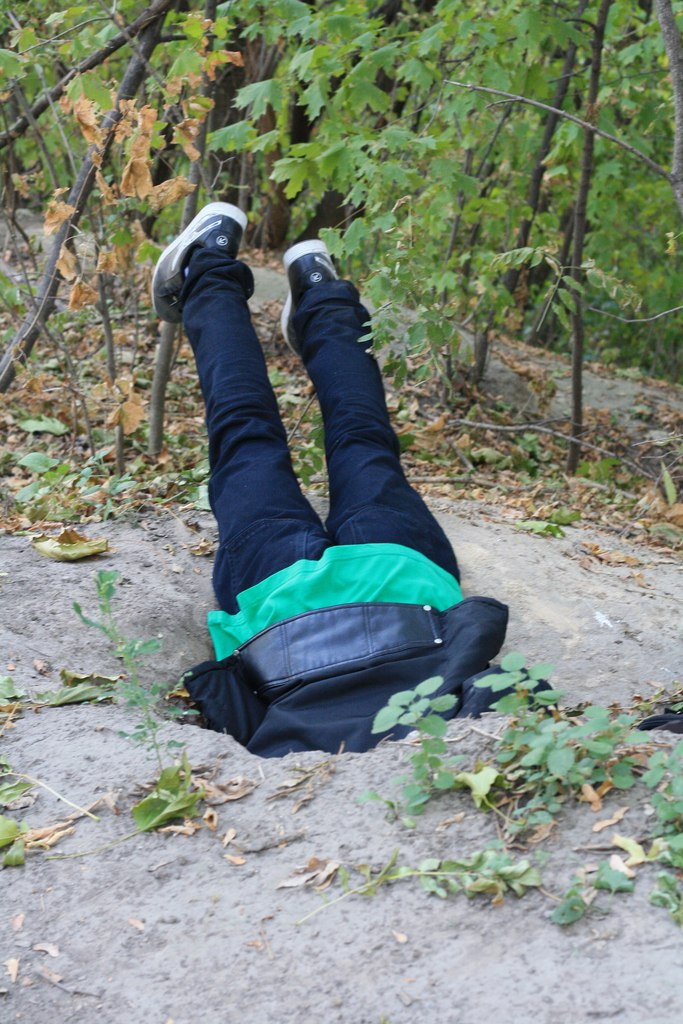
\includegraphics[width=0.65\linewidth]{chast-colebanie-osnov/gora-zamkovaya-valovaya/kraeved02.jpg}

\textit{Фото Алины Шиндировской.}
\end{center}

В 1876 году в усадьбе Кушнерева на Вознесенском спуске, в свертке истлевшего полотна нашли 200 серебряных монет Владимира Красна-Солнышка. Стоило ли древнему владельцу их зарывать? И чем тогда был Кудрявец – населенным районом или пустынью, чащобой дикой?

%Но Похилевич дает расстояние от Вознесенской церкви до развалин – 80 сажней на северо-запад, это 170 метров. На таком расстоянии отстоит от Художки южный корпус больницы Академии Наук. 

Однако, к тем раскопкам относится именно указанное мною место на мысу за больницей, ибо Лашкарев писал об окружении следующее:

\begin{quotation}
В пяти-шести саженях к западу и северо-западу начинается крутой обрыв ущелья, по которому идет так называемый вознесенский (иларионовский) спуск, дающий в этом пункте поворот к Подолу. Обрыв скрывал местность кургана\footnote{Под коим оказались развалины.} от всяких прохожих и придавал ей особый характер уединения. Ближайшая обстановка кургана, наводившая на мысль, что в нем есть что-то, привлекавшее к нему в былые времена внимание, уединенное и вместе выдающееся положение его на отроге горы, вдигающемся в промежуток, оставленный двумя другими, в преданиях знаменитыми киевскими горами – Щекавикою и Уздыхальницею\footnote{Путает Киселевку с Уздыхальницей.} [...]\end{quotation}

Этого достаточно, чтобы однозначно определить место раскопок, про которые писал Лашкарев, на мысу за больницей. А в усадьбе Художки – развалины Вознесенской или Спасской церквей.

\vspace*{\fill}

\begin{center}
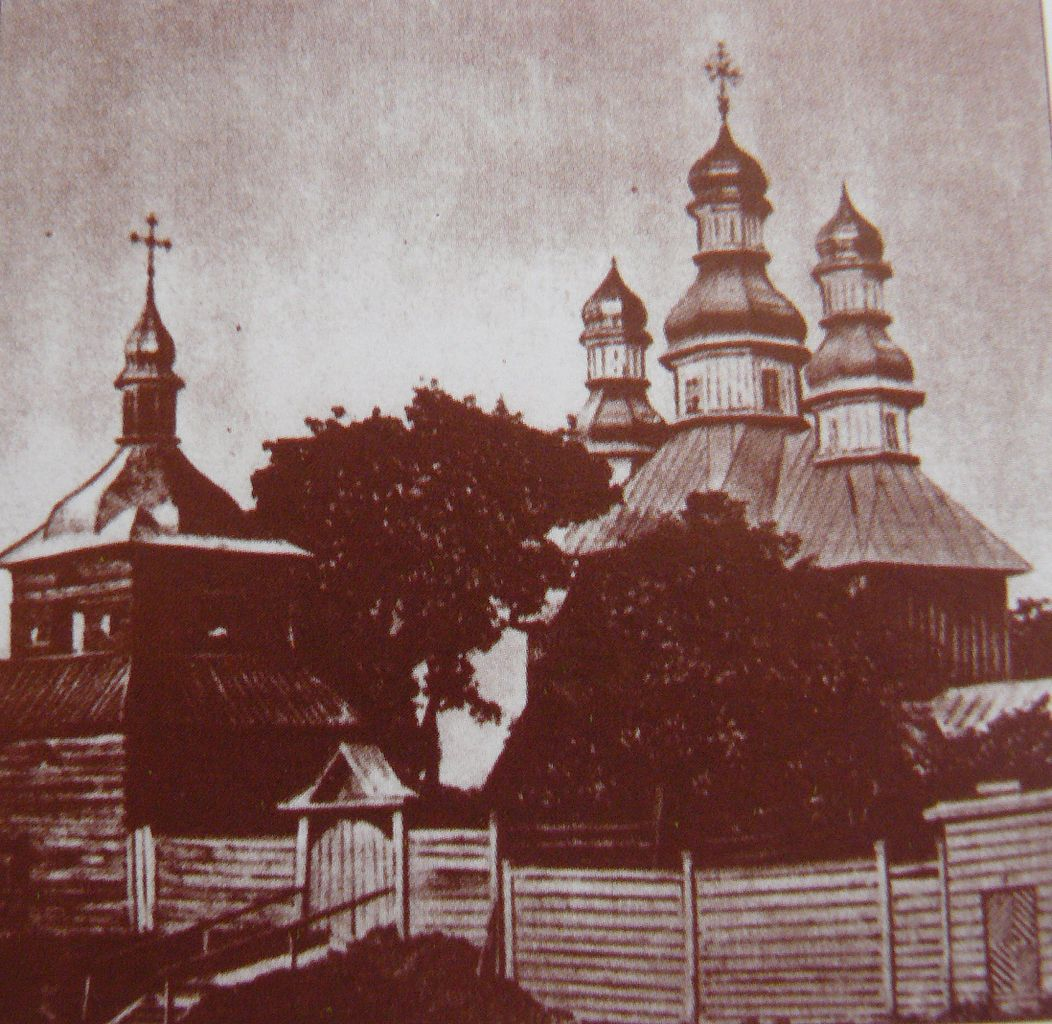
\includegraphics[width=0.85\linewidth]{chast-colebanie-osnov/gora-zamkovaya-valovaya/vozncerk.jpg}

\textit{19 век, старая Вознесенская церковь.}
\end{center}

\newpage
\begin{center}
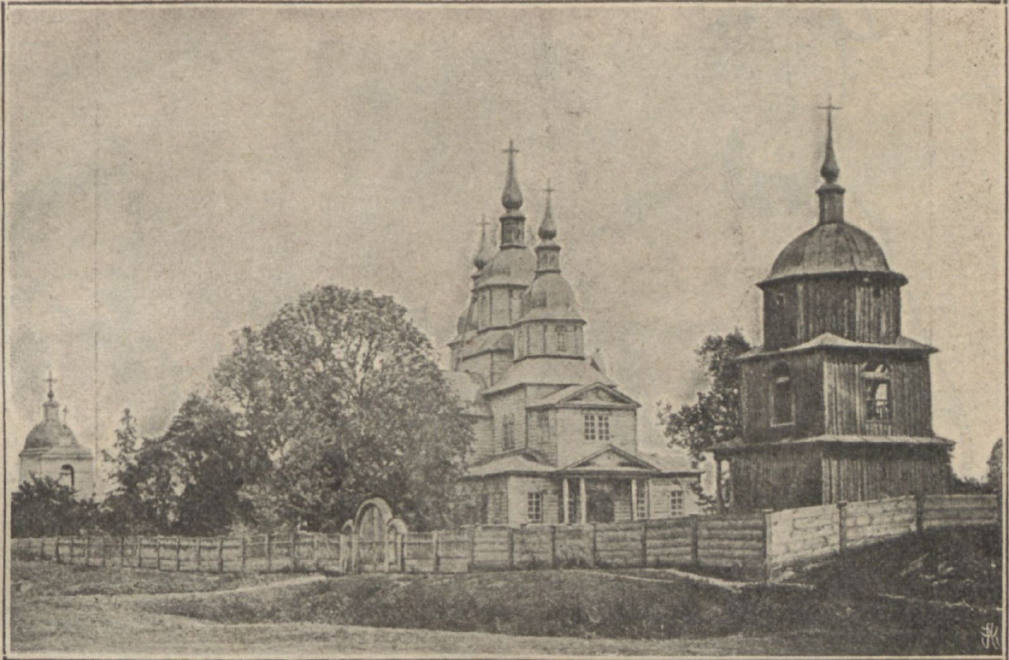
\includegraphics[width=0.94\linewidth]{chast-colebanie-osnov/gora-zamkovaya-valovaya/vozncerk02.jpg}

\textit{19 век, старая Вознесенская церковь, вид с другой стороны.}
\end{center}

\begin{center}
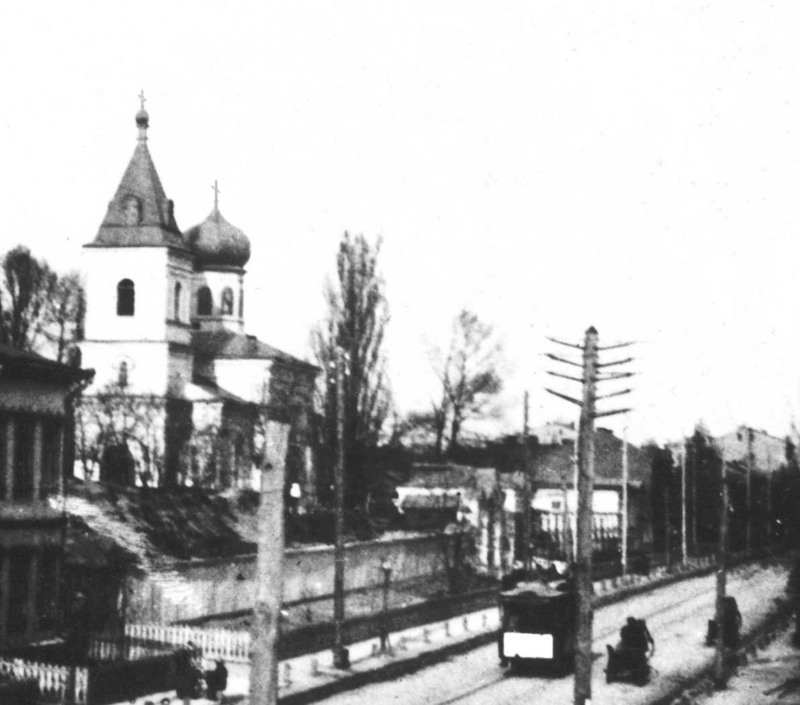
\includegraphics[width=0.94\linewidth]{chast-colebanie-osnov/gora-zamkovaya-valovaya/vozn-nov.jpg}

\textit{Новая Вознесенская церковь, на Дорогожицкой. Дореволюционный снимок.}
\end{center}
\newpage

Новая же Вознесенская церковь (снесена в 1930-х) и Вознесенское (Старокиевское) кладбище при ней находились там, где ныне усадьба на Артёма, 46. Сохранились только церковные ворота, они глядят в сторону улицы. 

Кладбище, бывшее там и до церкви, на стыке 19-20 веков простиралось к востоку от строений Покровского монастыря, внутри его стены, по склону до Дионисьева переулка (ныне Бехтеревского), что соединялся с Глубочицкой улицей. Теперь за воротами – особняк, построенный в 1948-м пленными венграми\footnote{Они вложили в стену капсулу с запиской: «Память: Киев, 1948, 10 февраля. Этот дом строили 20 человек венгерских военнопленных, это – их честная работа. Кто найдет эту записку – читая, вспомни о работе рук венгерского мужчины» – далее перечислялись фамилии.} для семьи генерала Ватутина, погибшего в 1944 году. Но вместо родичей Ватутина в доме поселился руководитель Совета писателей Украины, драматург Александр Корнейчук с женой, писательницей Вандой Василевской.

В 1863 году Вознесенский спуск переименовали в Илларионовский, по имени Киевского генерал-губернатора Иллариона Илларионовича Васильчикова (1805-1862), однако верхняя четная часть сохранила прежнее название до двадцатых годов двадцатого же века. Васильчиков удостоился такой чести, ибо по его распоряжению улицу вымостили брусчаткой. Если этот почин продолжать дальше, то все улицы Киева будут называться по фамилиям градоначальников, ибо каждый из них отдавал различные приказы по благоустройству дорог.

В Киеве, в пойме Сырца, есть также «дача Васильчикова», она же, позже стала очередной «дачей Хрущова» и прочих партийных боссов. По состоянию на 2021 год пребывает в диком запустении.

Но давайте пройдемся по Вознесенскому спуску! Некогда многолюдный, мощеный камнем, поглядим каков он ныне, примерно с половины, сверху вниз. Замечу, что когда я стал изредка посещать его в 2005, то застал еще, по левой стороне (противоположной к Художественной Академии), напротив больницы разрушенные старинные дома – остовы кирпичных стен, провалившиеся, бесформенные ржавые крыши, и всё это зарастало бурьяном. На 2015 год и следа их нет уже, держался только домик номер 21, и чуть ниже его – наполовину деревянный 23 (участок был выставлен на продажу, значит домику жить осталось недолго).

\begin{center}
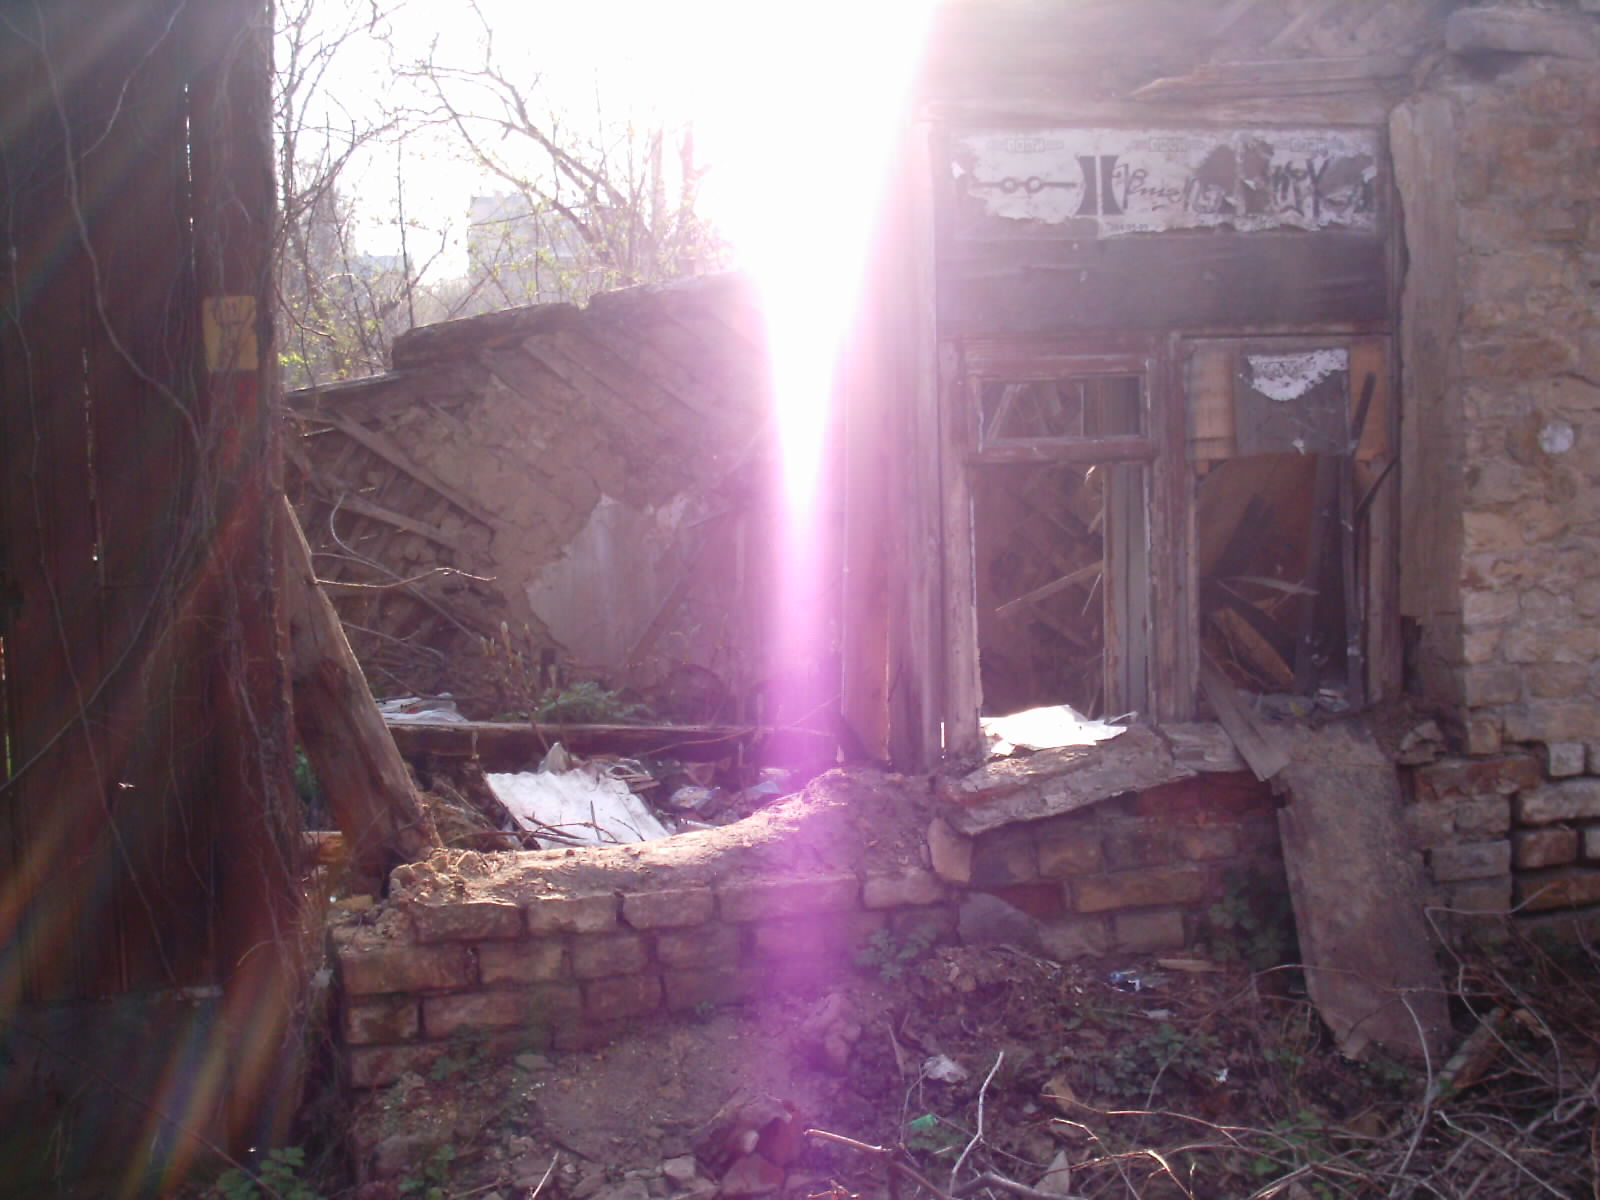
\includegraphics[width=0.86\linewidth]{chast-colebanie-osnov/gora-zamkovaya-valovaya/imag0013.jpg}

\textit{2005 год, никого нет дома.}
\end{center}

\begin{center}
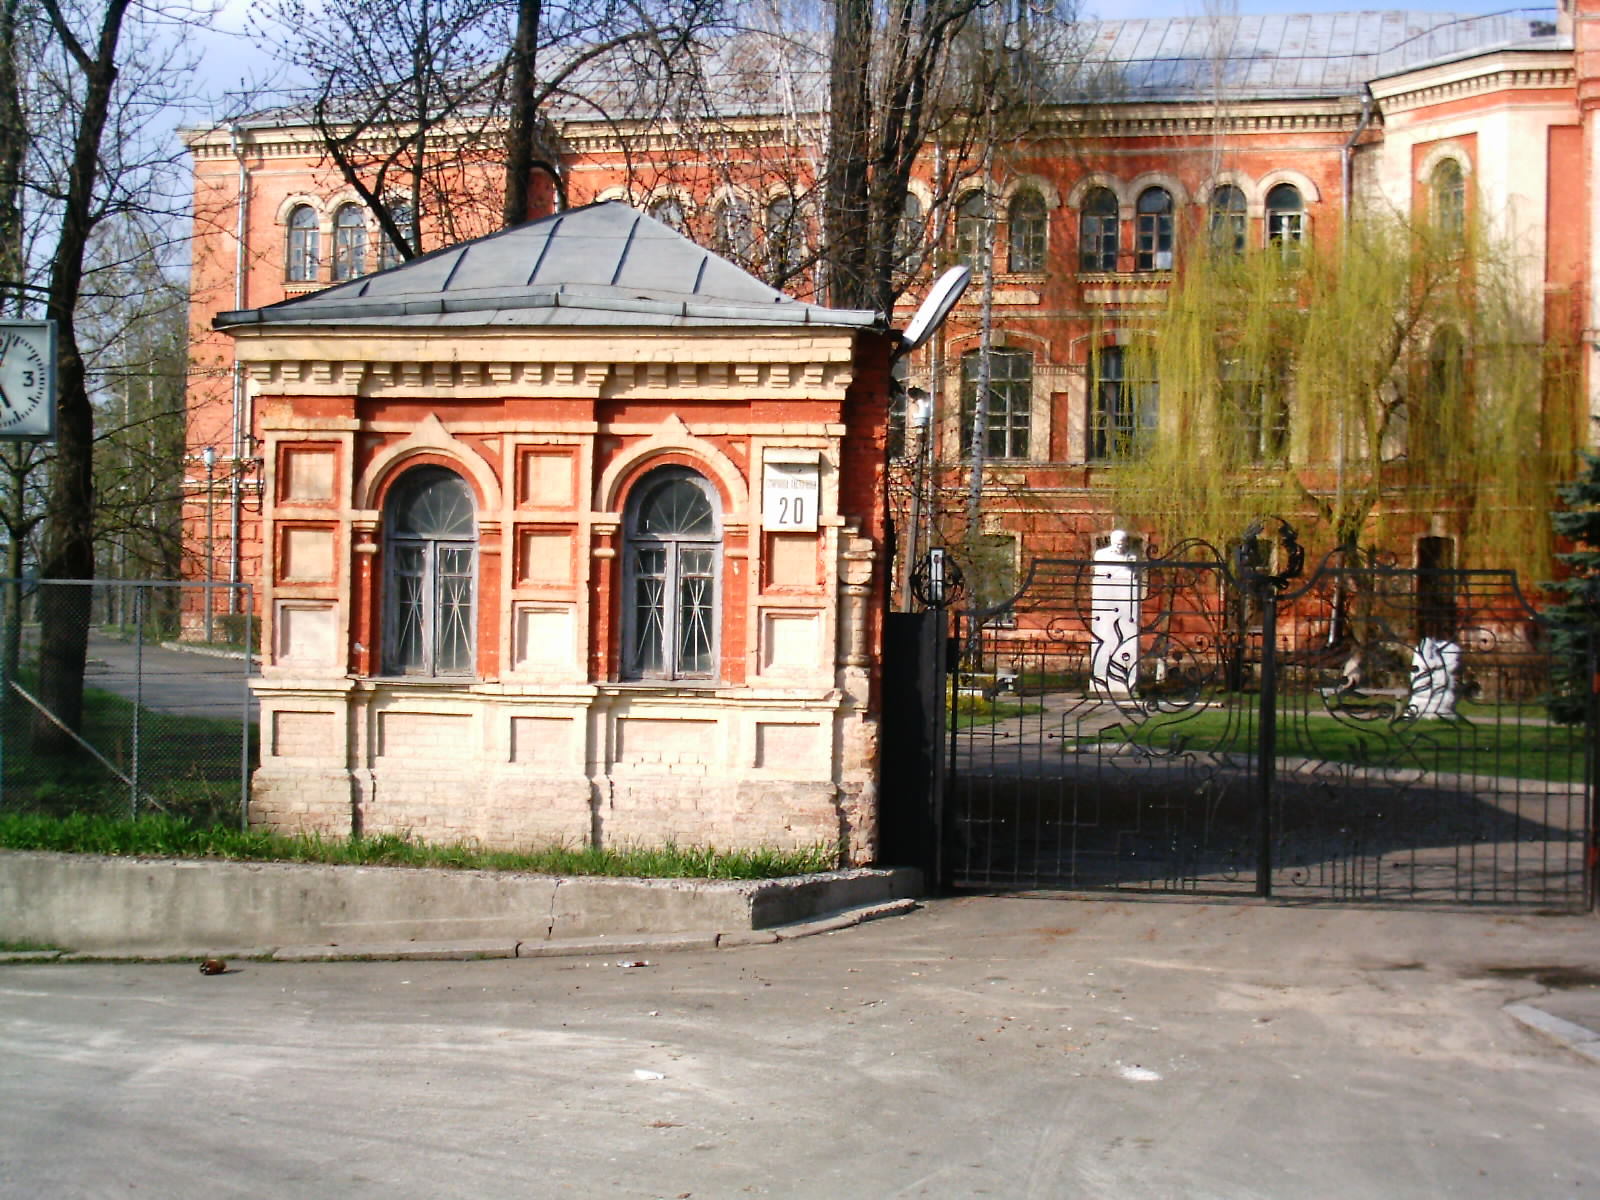
\includegraphics[width=0.86\linewidth]{chast-colebanie-osnov/gora-zamkovaya-valovaya/imag0006.jpg}

\textit{2005 год, Художественная академия.}
\end{center}

\newpage

\begin{center}
\includegraphics[width=\linewidth]{chast-colebanie-osnov/gora-zamkovaya-valovaya/\myimgprefix seminaria.jpg}

\textit{Там же, во время Первой мировой, в семинарии расположился лазарет.}
\end{center}

\begin{center}
\includegraphics[width=\linewidth]{chast-colebanie-osnov/gora-zamkovaya-valovaya/\myimgprefix IMG_4418.JPG}

\textit{2015. Домик по нечетной стороне улицы. Справа будет больницы, слева, за домиком, в яру улица Петровская, ранее Вознесенский яр.}
\end{center}

\newpage
\vspace*{\fill}
\begin{center}
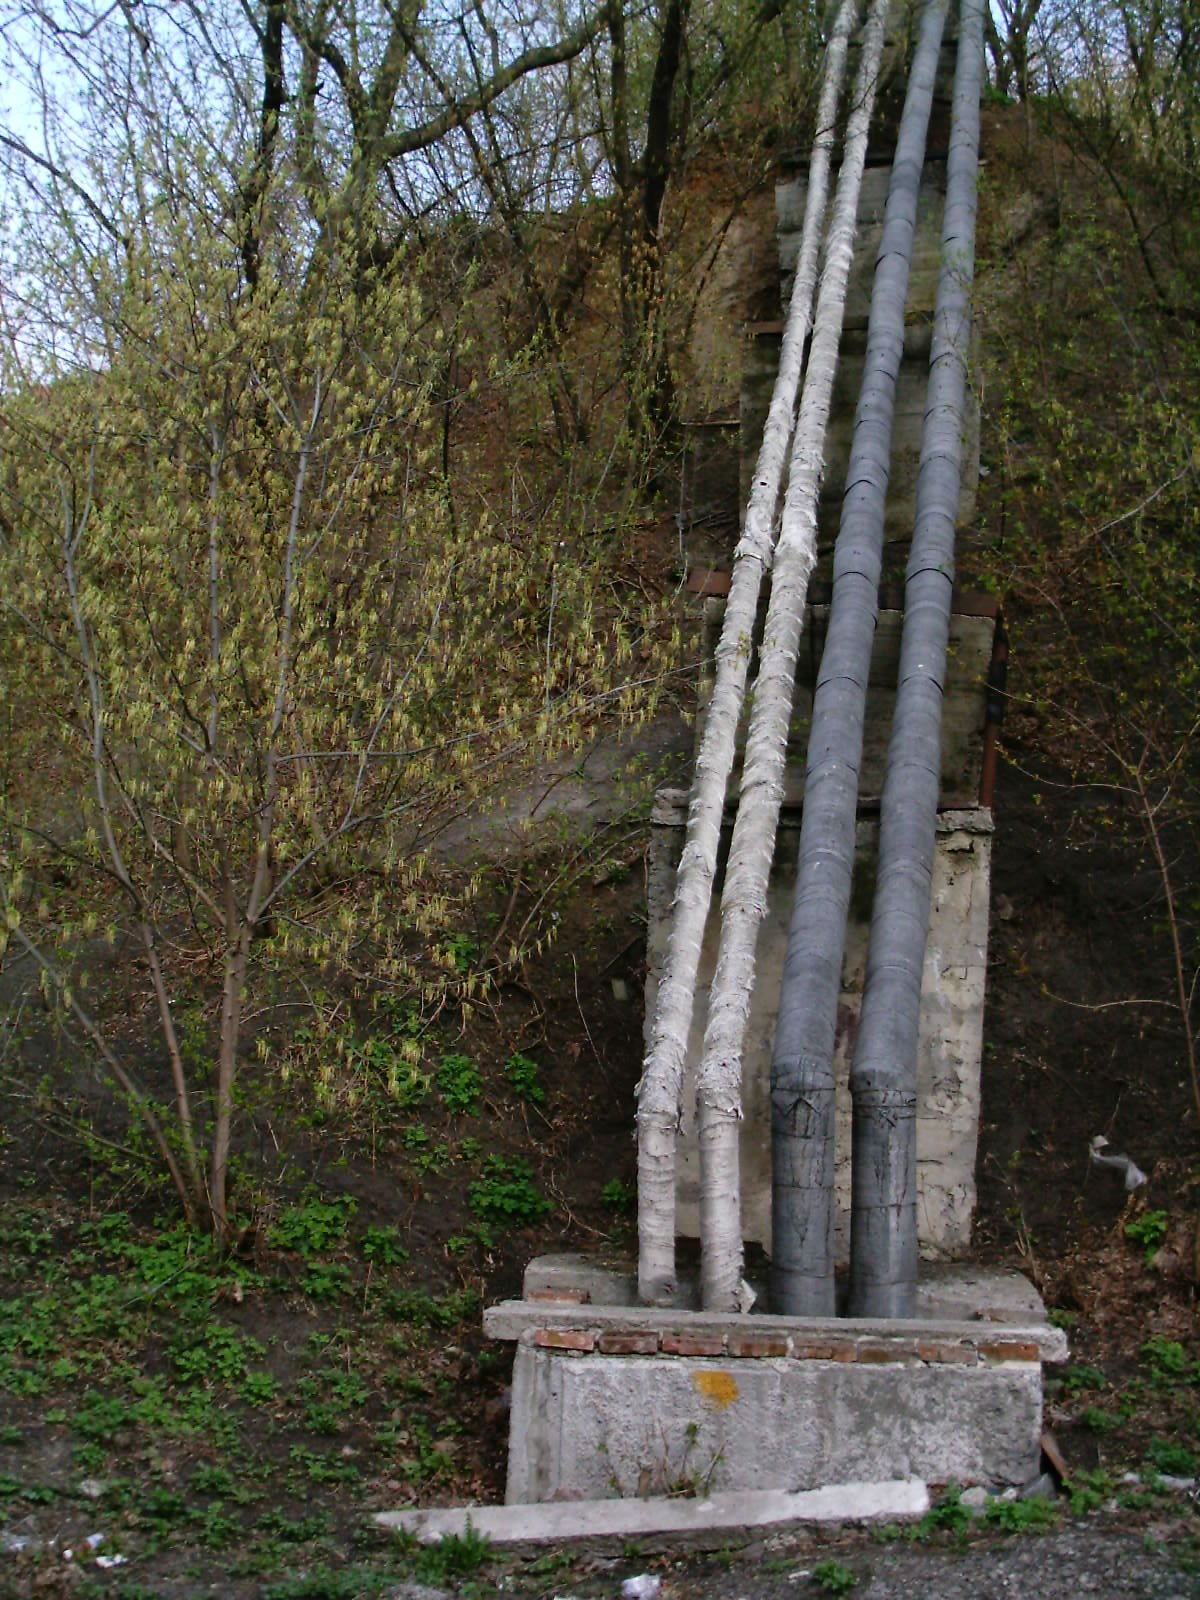
\includegraphics[width=\linewidth]{chast-colebanie-osnov/gora-zamkovaya-valovaya/imag0021.jpg}

\textit{2005 год, западный мыс холма с больницей.
Быть может, на этой круче и стояла церковь Симеона.}
\end{center}
\vspace*{\fill}
\newpage

\begin{center}
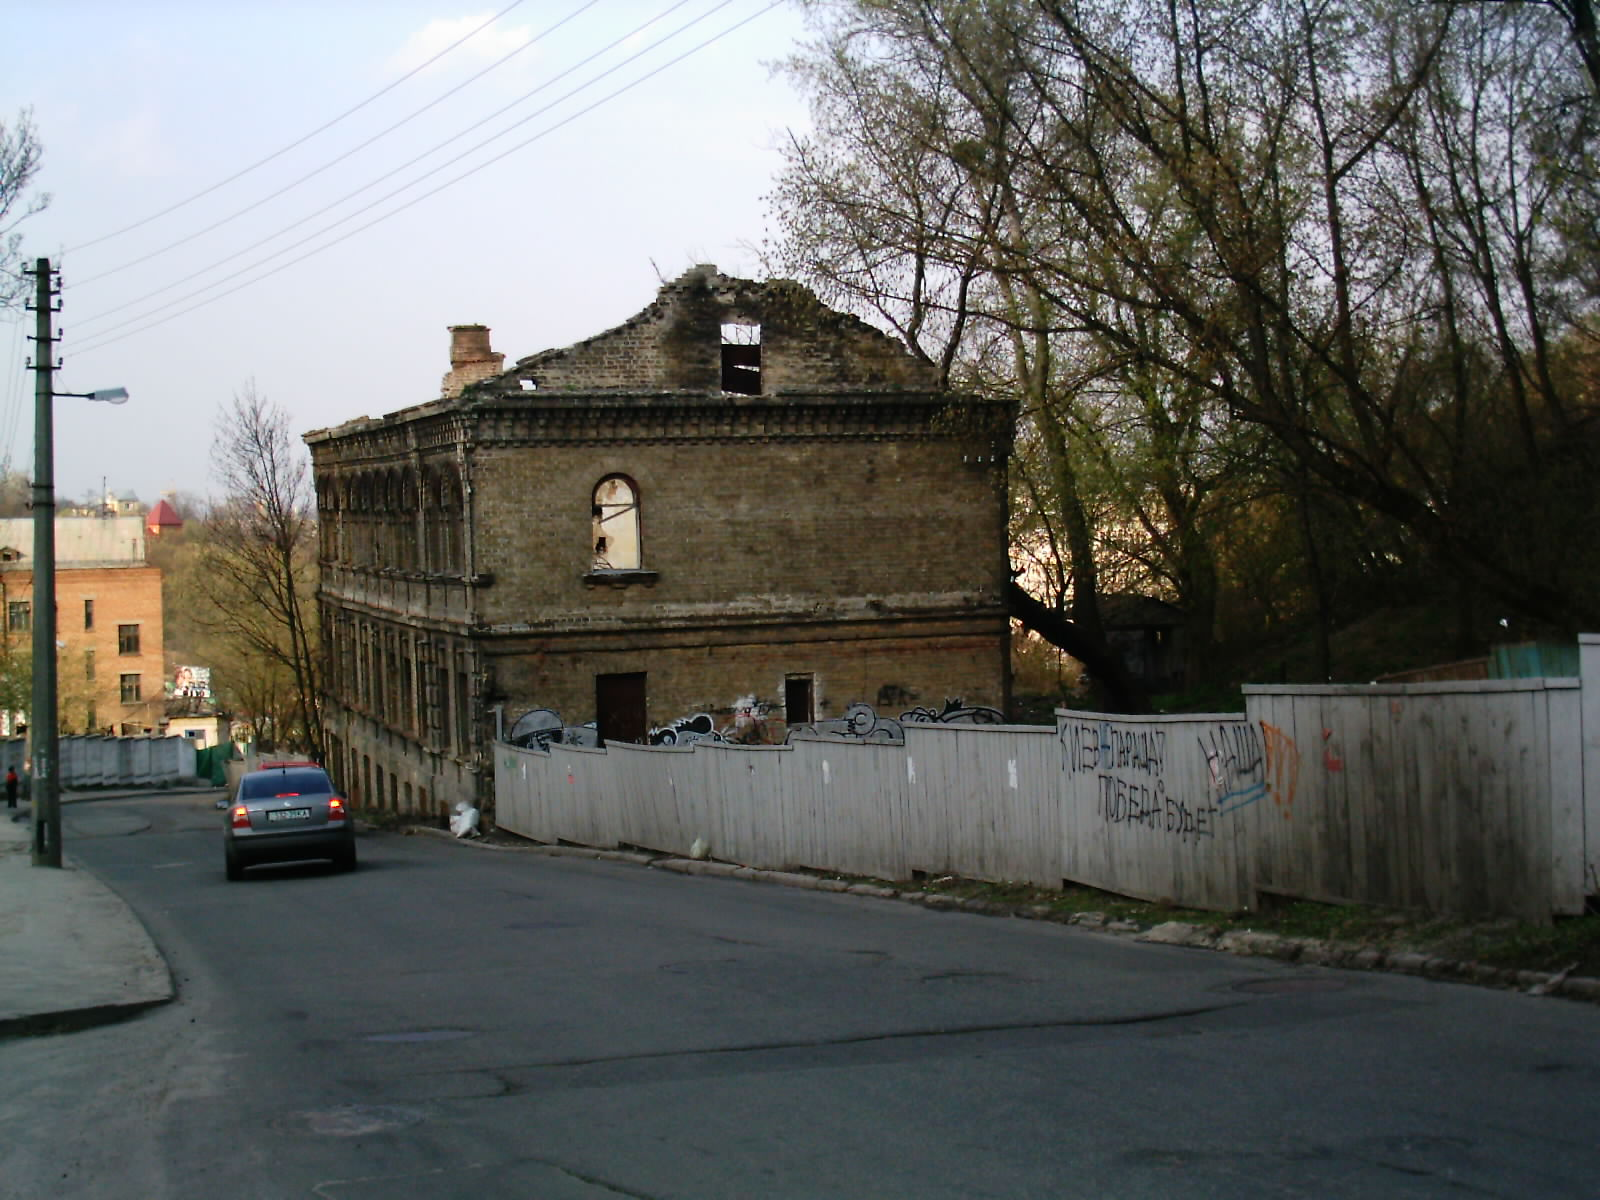
\includegraphics[width=\linewidth]{chast-colebanie-osnov/gora-zamkovaya-valovaya/imag0022.jpg}

\textit{2005 год, нижняя часть спуска, дом №26.}
\end{center}

\begin{center}
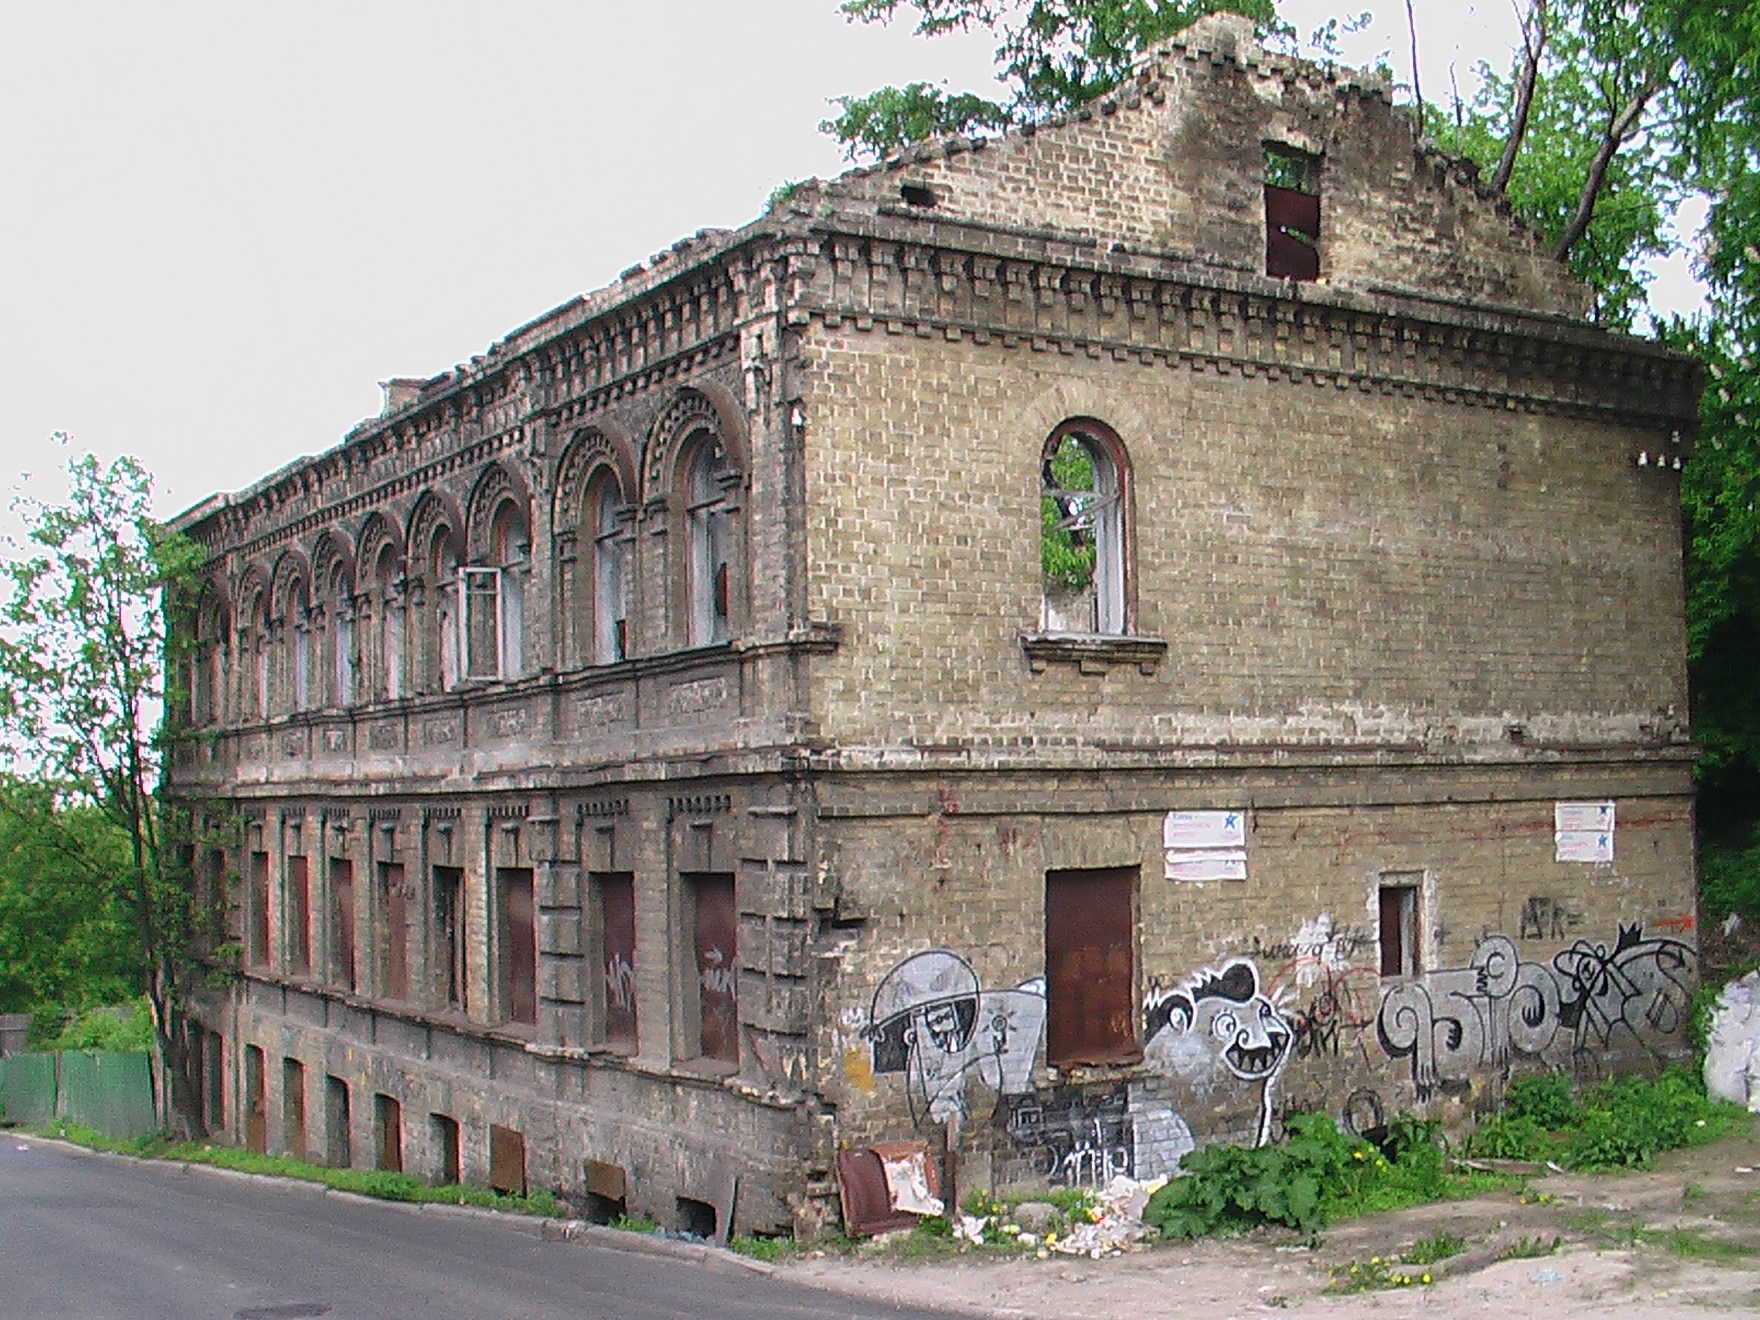
\includegraphics[width=\linewidth]{chast-colebanie-osnov/gora-zamkovaya-valovaya/imga0036.jpg}

\textit{2006 год, ближе.}
\end{center}

\newpage

\begin{center}
\includegraphics[width=\linewidth]{chast-colebanie-osnov/gora-zamkovaya-valovaya/\myimgprefix imga0037.jpg}

\textit{2006 год, украшения дома №26 крупно.}
\end{center}

\begin{center}
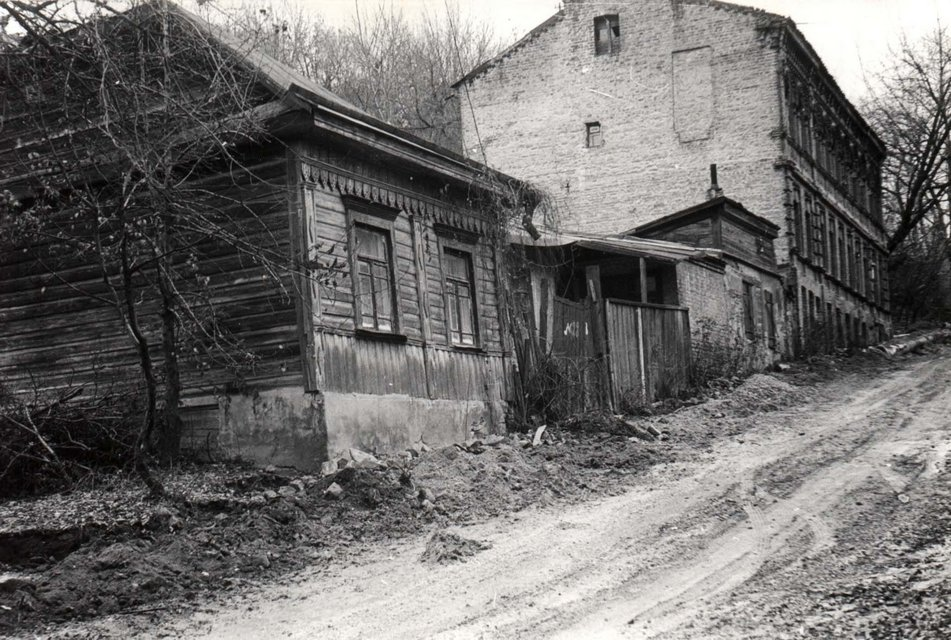
\includegraphics[width=\linewidth]{chast-colebanie-osnov/gora-zamkovaya-valovaya/vozn-2x.jpg}

\textit{Тот же дом в незапамятное время, вид снизу улицы вверх.}
\end{center}

\newpage
\vspace*{\fill}
\begin{center}
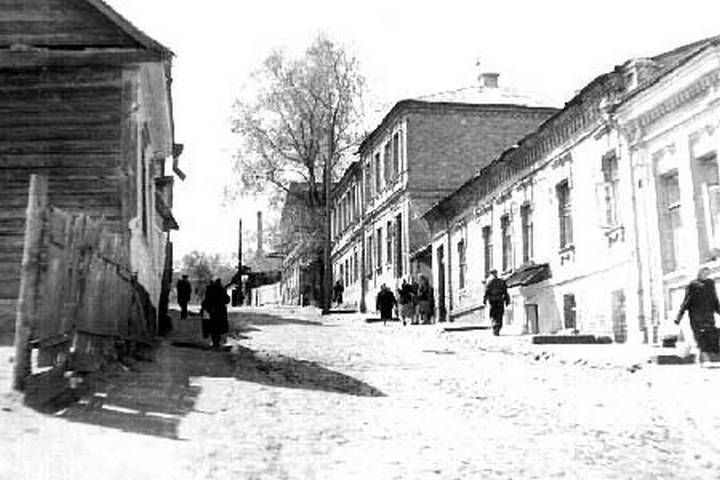
\includegraphics[width=\linewidth]{chast-colebanie-osnov/gora-zamkovaya-valovaya/vozn-drug.jpg}

\textit{В незапамятное время глядим оттуда правее.}
\end{center}


\begin{center}
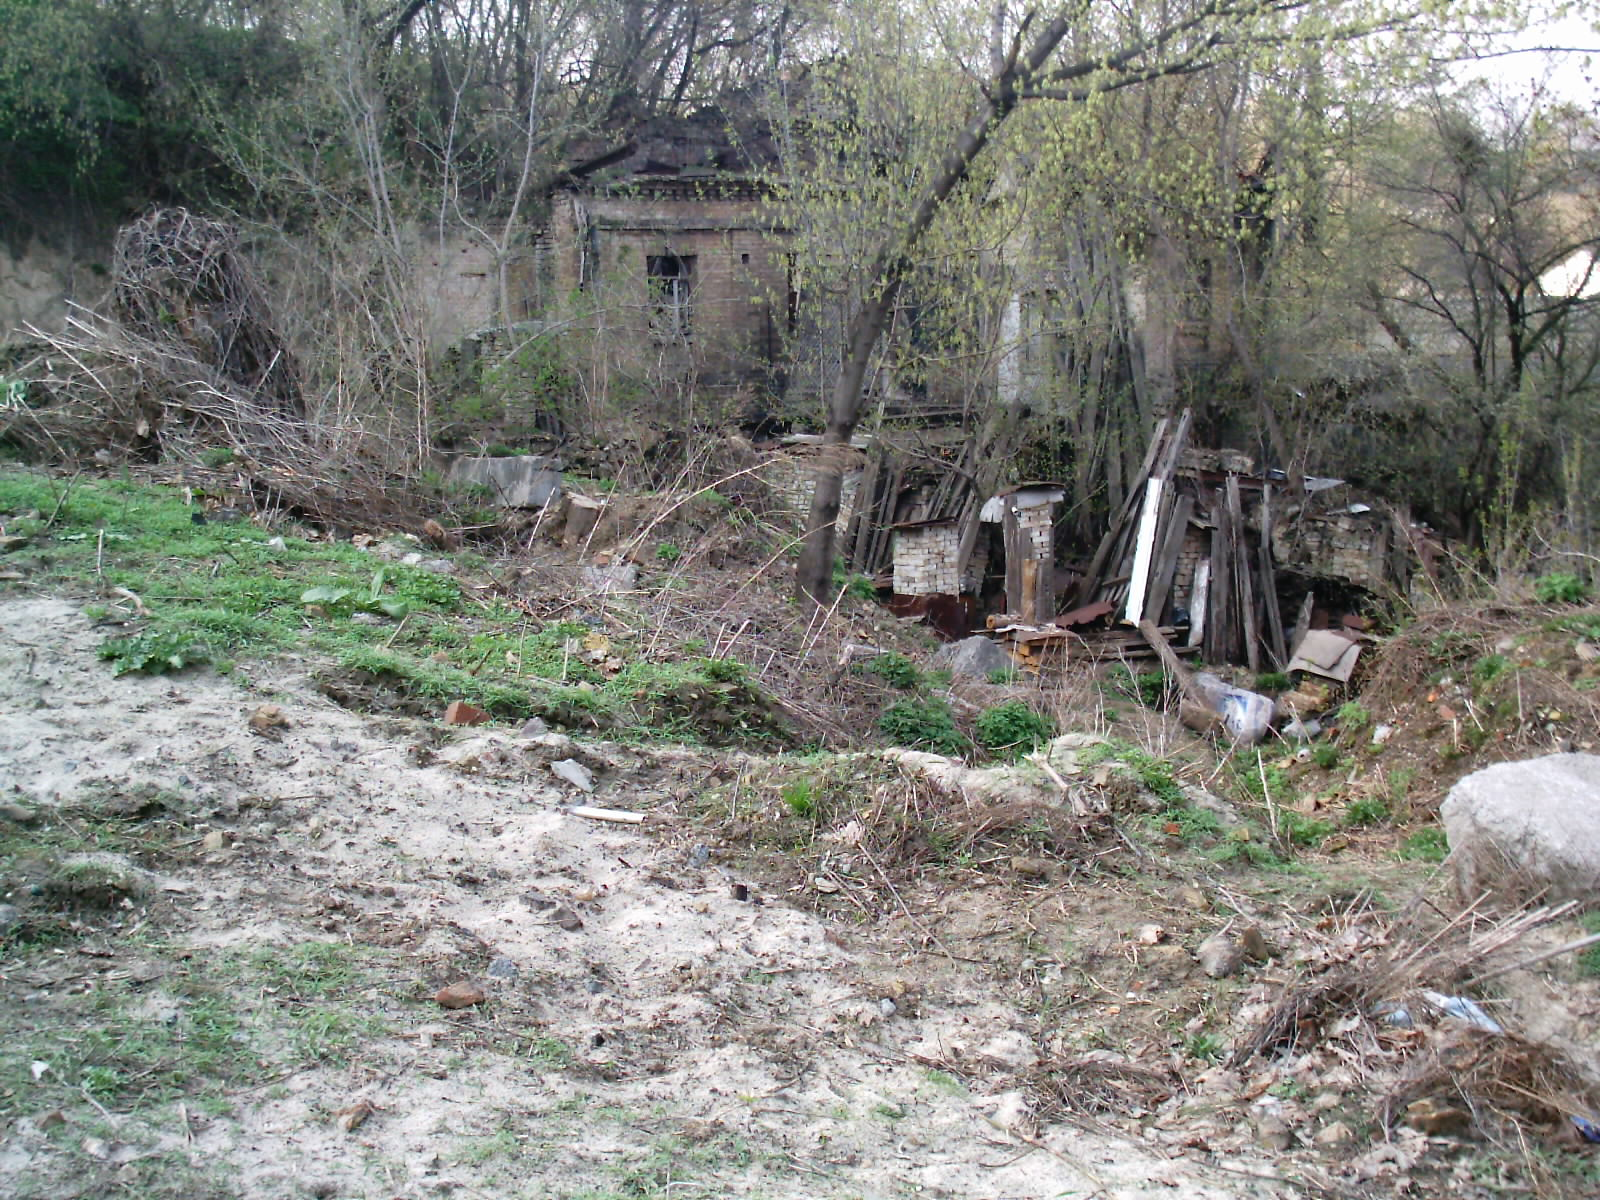
\includegraphics[width=\linewidth]{chast-colebanie-osnov/gora-zamkovaya-valovaya/imag0024.jpg}

\textit{И 2005 год, там же, по нечетной стороне.}
\end{center}
\vspace*{\fill}
\newpage

\begin{center}
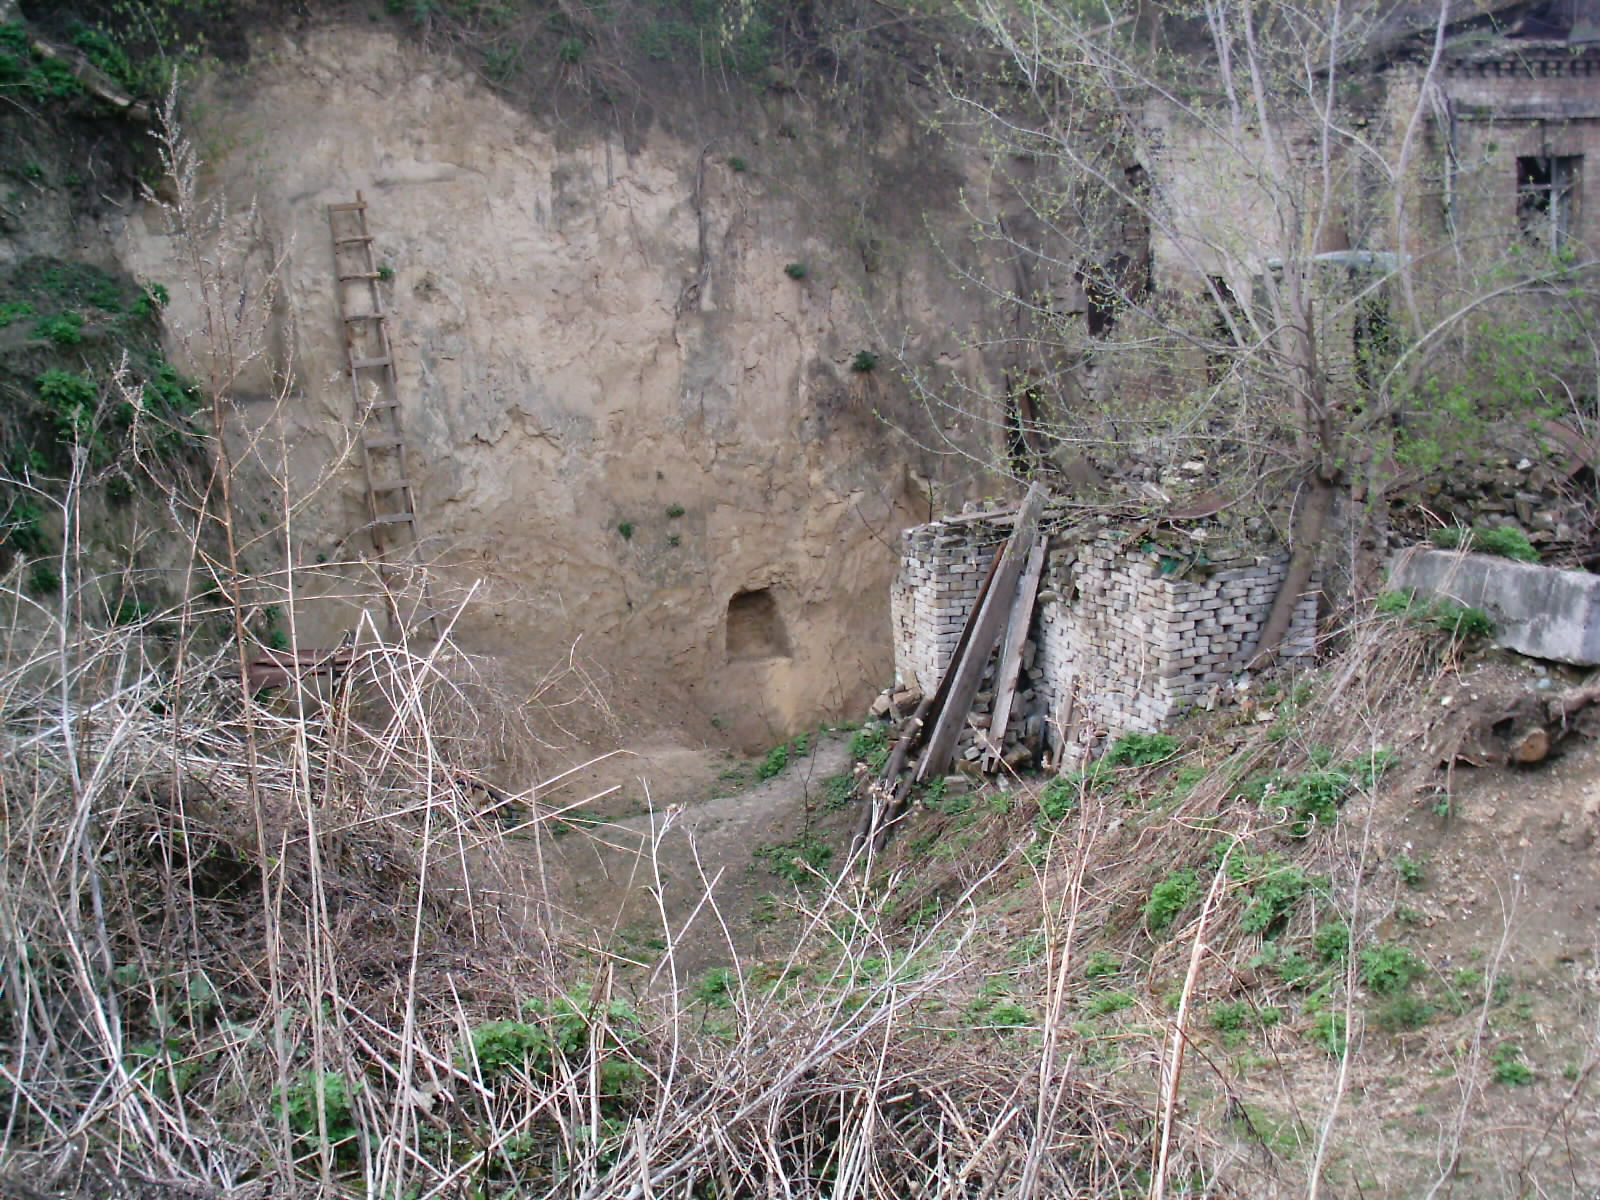
\includegraphics[width=\linewidth]{chast-colebanie-osnov/gora-zamkovaya-valovaya/imag0025.jpg}

\textit{2005 год, там же.}
\end{center}

\begin{center}
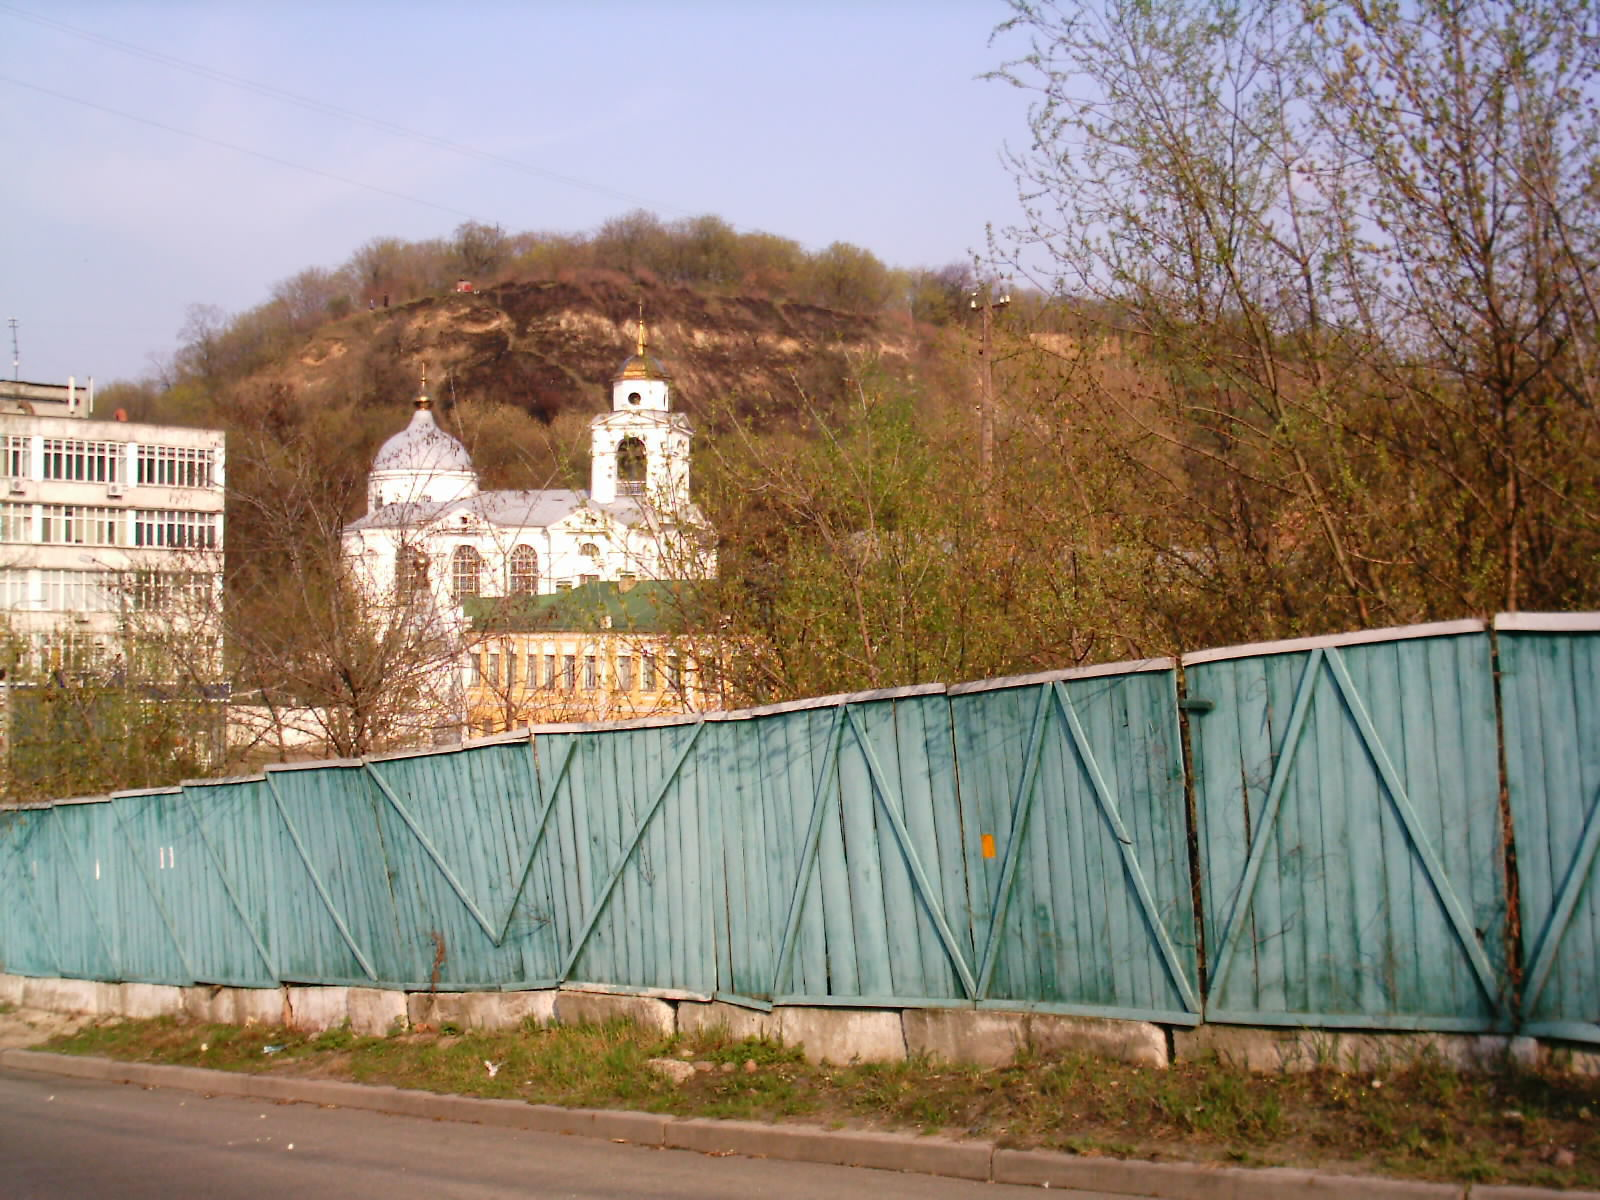
\includegraphics[width=\linewidth]{chast-colebanie-osnov/gora-zamkovaya-valovaya/imag0026.jpg}

\textit{2005 год, вид на Замковую с Вознесенского спуска.}
\end{center}

\begin{center}
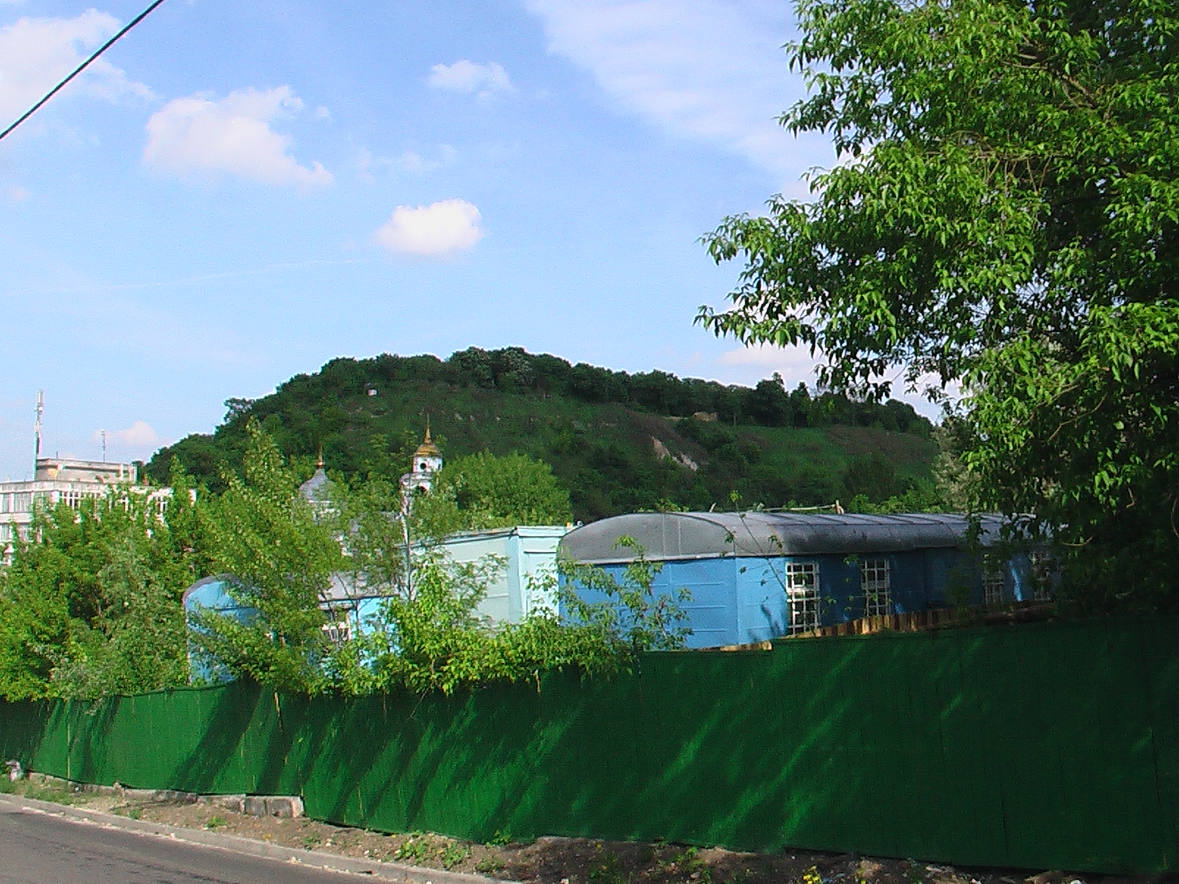
\includegraphics[width=\linewidth]{chast-colebanie-osnov/gora-zamkovaya-valovaya/s_imga0041.jpg}

\textit{2006 год, вид на Замковую с Вознесенского спуска.}
\end{center}

На фотографии, где окна выпотрошенного, горелого дома показаны крупно – одна створка еще отворена. Чьи-то руки открывали ее десятки, а скорее сотню лет, на подоконнике стояли цветы, а за косяком проглядывали не деревья с небом, но жилая комната. 

Сейчас Вознесенский спуск застраивается, что сложно, ибо с четной стороны негде, а с нечетной – Вознесенский яр, в котором проложена Петровская улица (до 1907 года – улица Вознесенский Яр), ныне обрезанная в южной части.

Примечательно, что через улицу, напротив мыса (в сторону кинологического центра), в противоположном, тоже суглинном склоне, была или есть пещера, но я не видел ее. Судя по косвенным данным осени 2022 года, этот бывший адрес Вознесенский спуск, 25, упомянут как место наличия пещер 12 века, и его собираются застроить. На осень 2022 года там пустырь, снесенное старое жилье, кое-какие постройки уцелели, виден также обнаженный суглинный, почти отвесный склон, к которому вероятно примыкал вплотную дом, ныне разваленный. Там котлован, внизу заросшие зеленью балки, перекрытия, и одна из стен котлована вырастает эдаким ровным лёссовым обрывом. Кажется, бывшее там строение уходило на один этаж или даже несколько под землю. Мы с друзьями снимали там одну из сцен любительского фильма «Школа», как раз про археологические раскопки, не зная в то время совершенно о близлежащей пещере.

В таком состоянии я наблюдал это, попадая туда время от времени с середины нулевых.

Не знаю, о той же ли самой, или другой пещере, в октябре 2022 года сообщил в Facebook Тимур Бобровский – он написал, что на Вознесенском спуске есть пещера длиной 40 метров, по конфигурации и архитектуре подобная Змиевой на Смородинском спуске. На приведенных им фотографиях видно следующее. На одной – прямоугольный в сечении коридор в лёссе, чистый, без следов влаги, с некими двойными полосами в стенах ближе к полу, на одинаковой высоте с обеих сторон, с грубо выделанным потолком. 

На другом снимке сам вход в пещеру, нора в полукруглой пазухе, невесть в каком склоне – небольшой обрывчик (видимость метра два с вершком от норы до верха), замшелый суглинок, сверху спускается корень дерева, под корнем виден кирпич, над входом в суглинке торчит кирпич, левее вообще сегмент кирпичной стены, по снимку трудно разобрать старинные они или нет. В комментах написано, что у пещеры есть и другой вход.

За этим последовала статья, где сказано, что там четыре пещеры, входы в две засыпаны. Об одной из доступных, длиной около «35 метров» сообщается, что на стенах есть «анимистические» и более поздние «варяжского периода» граффити.
   
...На последних фотографиях в этой главе мы почти спустились к бывшей Кожемяцкой площади, перекрестку с Глубочицкой улицей. Глядим на восток и видим гору Киселёвку с Воздвиженской церковью под нею. Однако нам в иную сторону, налево. От горы Воловни, пересечем улицу Глубочицкую к подножию другой горы – Щекавицы.